\documentclass[twoside]{book}

% Packages required by doxygen
\usepackage{fixltx2e}
\usepackage{calc}
\usepackage{doxygen}
\usepackage[export]{adjustbox} % also loads graphicx
\usepackage{graphicx}
\usepackage[utf8]{inputenc}
\usepackage{makeidx}
\usepackage{multicol}
\usepackage{multirow}
\PassOptionsToPackage{warn}{textcomp}
\usepackage{textcomp}
\usepackage[nointegrals]{wasysym}
\usepackage[table]{xcolor}

% Font selection
\usepackage[T1]{fontenc}
\usepackage[scaled=.90]{helvet}
\usepackage{courier}
\usepackage{amssymb}
\usepackage{sectsty}
\renewcommand{\familydefault}{\sfdefault}
\allsectionsfont{%
  \fontseries{bc}\selectfont%
  \color{darkgray}%
}
\renewcommand{\DoxyLabelFont}{%
  \fontseries{bc}\selectfont%
  \color{darkgray}%
}
\newcommand{\+}{\discretionary{\mbox{\scriptsize$\hookleftarrow$}}{}{}}

% Page & text layout
\usepackage{geometry}
\geometry{%
  a4paper,%
  top=2.5cm,%
  bottom=2.5cm,%
  left=2.5cm,%
  right=2.5cm%
}
\tolerance=750
\hfuzz=15pt
\hbadness=750
\setlength{\emergencystretch}{15pt}
\setlength{\parindent}{0cm}
\setlength{\parskip}{3ex plus 2ex minus 2ex}
\makeatletter
\renewcommand{\paragraph}{%
  \@startsection{paragraph}{4}{0ex}{-1.0ex}{1.0ex}{%
    \normalfont\normalsize\bfseries\SS@parafont%
  }%
}
\renewcommand{\subparagraph}{%
  \@startsection{subparagraph}{5}{0ex}{-1.0ex}{1.0ex}{%
    \normalfont\normalsize\bfseries\SS@subparafont%
  }%
}
\makeatother

% Headers & footers
\usepackage{fancyhdr}
\pagestyle{fancyplain}
\fancyhead[LE]{\fancyplain{}{\bfseries\thepage}}
\fancyhead[CE]{\fancyplain{}{}}
\fancyhead[RE]{\fancyplain{}{\bfseries\leftmark}}
\fancyhead[LO]{\fancyplain{}{\bfseries\rightmark}}
\fancyhead[CO]{\fancyplain{}{}}
\fancyhead[RO]{\fancyplain{}{\bfseries\thepage}}
\fancyfoot[LE]{\fancyplain{}{}}
\fancyfoot[CE]{\fancyplain{}{}}
\fancyfoot[RE]{\fancyplain{}{\bfseries\scriptsize Generated by Doxygen }}
\fancyfoot[LO]{\fancyplain{}{\bfseries\scriptsize Generated by Doxygen }}
\fancyfoot[CO]{\fancyplain{}{}}
\fancyfoot[RO]{\fancyplain{}{}}
\renewcommand{\footrulewidth}{0.4pt}
\renewcommand{\chaptermark}[1]{%
  \markboth{#1}{}%
}
\renewcommand{\sectionmark}[1]{%
  \markright{\thesection\ #1}%
}

% Indices & bibliography
\usepackage{natbib}
\usepackage[titles]{tocloft}
\setcounter{tocdepth}{3}
\setcounter{secnumdepth}{5}
\makeindex

% Hyperlinks (required, but should be loaded last)
\usepackage{ifpdf}
\ifpdf
  \usepackage[pdftex,pagebackref=true]{hyperref}
\else
  \usepackage[ps2pdf,pagebackref=true]{hyperref}
\fi
\hypersetup{%
  colorlinks=true,%
  linkcolor=blue,%
  citecolor=blue,%
  unicode%
}

% Custom commands
\newcommand{\clearemptydoublepage}{%
  \newpage{\pagestyle{empty}\cleardoublepage}%
}

\usepackage{caption}
\captionsetup{labelsep=space,justification=centering,font={bf},singlelinecheck=off,skip=4pt,position=top}

%===== C O N T E N T S =====

\begin{document}

% Titlepage & ToC
\hypersetup{pageanchor=false,
             bookmarksnumbered=true,
             pdfencoding=unicode
            }
\pagenumbering{alph}
\begin{titlepage}
\vspace*{7cm}
\begin{center}%
{\Large Seniors Gone Wild }\\
\vspace*{1cm}
{\large Generated by Doxygen 1.8.14}\\
\end{center}
\end{titlepage}
\clearemptydoublepage
\pagenumbering{roman}
\tableofcontents
\clearemptydoublepage
\pagenumbering{arabic}
\hypersetup{pageanchor=true}

%--- Begin generated contents ---
\chapter{Hierarchical Index}
\section{Class Hierarchy}
This inheritance list is sorted roughly, but not completely, alphabetically\+:\begin{DoxyCompactList}
\item I\+Comparable\begin{DoxyCompactList}
\item \contentsline{section}{High\+Score}{\pageref{class_high_score}}{}
\end{DoxyCompactList}
\item Mono\+Behaviour\begin{DoxyCompactList}
\item \contentsline{section}{Audio\+Manager}{\pageref{class_audio_manager}}{}
\item \contentsline{section}{Camera\+Controller}{\pageref{class_camera_controller}}{}
\item \contentsline{section}{Exit\+Game}{\pageref{class_exit_game}}{}
\item \contentsline{section}{High\+Score\+Manager}{\pageref{class_high_score_manager}}{}
\item \contentsline{section}{High\+Score\+Script}{\pageref{class_high_score_script}}{}
\item \contentsline{section}{Load\+Credits}{\pageref{class_load_credits}}{}
\item \contentsline{section}{Load\+Escape\+Scene}{\pageref{class_load_escape_scene}}{}
\item \contentsline{section}{Load\+High\+Scores}{\pageref{class_load_high_scores}}{}
\item \contentsline{section}{Load\+New\+Area}{\pageref{class_load_new_area}}{}
\item \contentsline{section}{Load\+To\+Main}{\pageref{class_load_to_main}}{}
\item \contentsline{section}{Menu\+Script}{\pageref{class_menu_script}}{}
\item \contentsline{section}{Nurse\+Controller}{\pageref{class_nurse_controller}}{}
\item \contentsline{section}{Player\+Controller}{\pageref{class_player_controller}}{}
\item \contentsline{section}{Player\+Start\+Point}{\pageref{class_player_start_point}}{}
\item \contentsline{section}{Quit\+Button}{\pageref{class_quit_button}}{}
\end{DoxyCompactList}
\item \contentsline{section}{Sound}{\pageref{class_sound}}{}
\end{DoxyCompactList}

\chapter{Class Index}
\section{Class List}
Here are the classes, structs, unions and interfaces with brief descriptions\+:\begin{DoxyCompactList}
\item\contentsline{section}{\mbox{\hyperlink{class_audio_manager}{Audio\+Manager}} \\*This script is for controlling the game audio }{\pageref{class_audio_manager}}{}
\item\contentsline{section}{\mbox{\hyperlink{class_camera_controller}{Camera\+Controller}} }{\pageref{class_camera_controller}}{}
\item\contentsline{section}{\mbox{\hyperlink{class_exit_game}{Exit\+Game}} }{\pageref{class_exit_game}}{}
\item\contentsline{section}{\mbox{\hyperlink{class_high_score}{High\+Score}} \\*Creates Score, Name, and ID variables for the database I\+Comparable command used for sorthing the scores }{\pageref{class_high_score}}{}
\item\contentsline{section}{\mbox{\hyperlink{class_high_score_manager}{High\+Score\+Manager}} }{\pageref{class_high_score_manager}}{}
\item\contentsline{section}{\mbox{\hyperlink{class_high_score_script}{High\+Score\+Script}} \\*This script controls the scoreboard and adds information to it. (Like Player name, rank and score) }{\pageref{class_high_score_script}}{}
\item\contentsline{section}{\mbox{\hyperlink{class_load_credits}{Load\+Credits}} }{\pageref{class_load_credits}}{}
\item\contentsline{section}{\mbox{\hyperlink{class_load_escape_scene}{Load\+Escape\+Scene}} }{\pageref{class_load_escape_scene}}{}
\item\contentsline{section}{\mbox{\hyperlink{class_load_high_scores}{Load\+High\+Scores}} }{\pageref{class_load_high_scores}}{}
\item\contentsline{section}{\mbox{\hyperlink{class_load_new_area}{Load\+New\+Area}} }{\pageref{class_load_new_area}}{}
\item\contentsline{section}{\mbox{\hyperlink{class_load_to_main}{Load\+To\+Main}} }{\pageref{class_load_to_main}}{}
\item\contentsline{section}{\mbox{\hyperlink{class_menu_script}{Menu\+Script}} }{\pageref{class_menu_script}}{}
\item\contentsline{section}{\mbox{\hyperlink{class_nurse_controller}{Nurse\+Controller}} }{\pageref{class_nurse_controller}}{}
\item\contentsline{section}{\mbox{\hyperlink{class_player_controller}{Player\+Controller}} }{\pageref{class_player_controller}}{}
\item\contentsline{section}{\mbox{\hyperlink{class_player_start_point}{Player\+Start\+Point}} }{\pageref{class_player_start_point}}{}
\item\contentsline{section}{\mbox{\hyperlink{class_quit_button}{Quit\+Button}} }{\pageref{class_quit_button}}{}
\item\contentsline{section}{\mbox{\hyperlink{class_sound}{Sound}} \\*This is necessary for getting access to audio settings like volume and pitch this will give this class a permission to appear in the inspector }{\pageref{class_sound}}{}
\end{DoxyCompactList}

\chapter{Class Documentation}
\hypertarget{class_audio_manager}{}\section{Audio\+Manager Class Reference}
\label{class_audio_manager}\index{Audio\+Manager@{Audio\+Manager}}


This script is for controlling the game audio  


Inheritance diagram for Audio\+Manager\+:\begin{figure}[H]
\begin{center}
\leavevmode
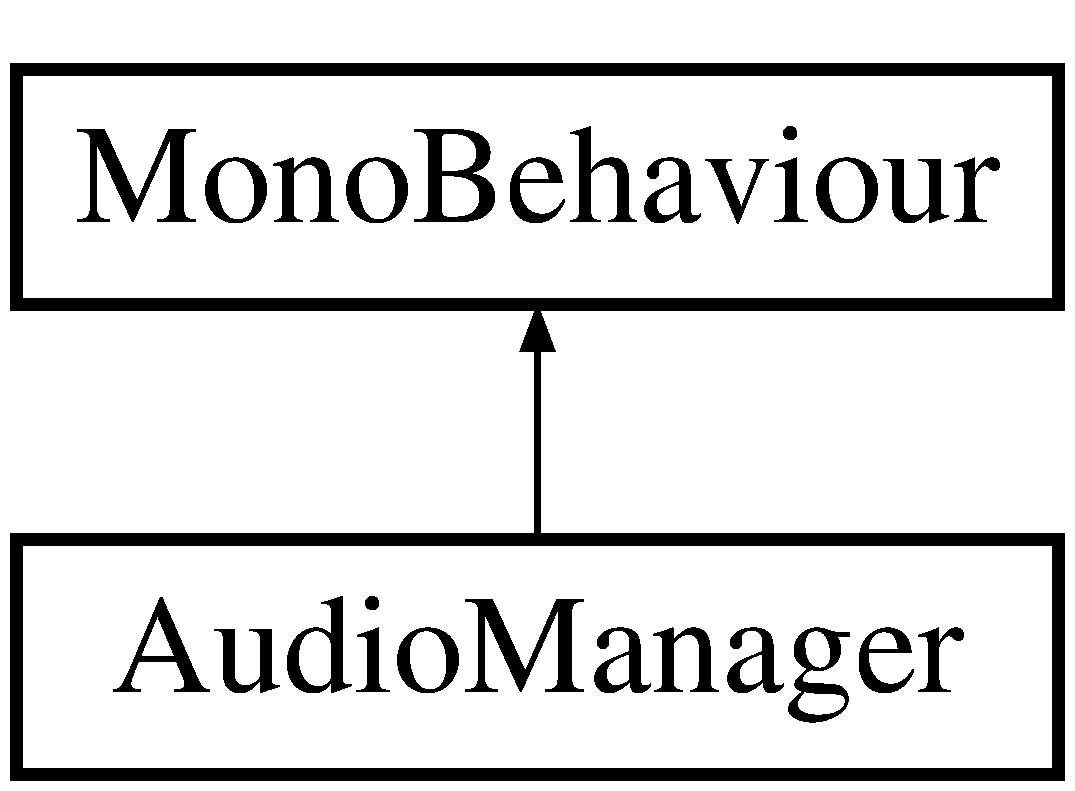
\includegraphics[height=2.000000cm]{class_audio_manager}
\end{center}
\end{figure}
\subsection*{Public Member Functions}
\begin{DoxyCompactItemize}
\item 
void \mbox{\hyperlink{class_audio_manager_a51d560f729b1fd4d6b5ce83ca558deb2}{Play}} (string name)
\begin{DoxyCompactList}\small\item\em This is for other classes to find their own sound from the audio manager \end{DoxyCompactList}\end{DoxyCompactItemize}
\subsection*{Public Attributes}
\begin{DoxyCompactItemize}
\item 
\mbox{\hyperlink{class_sound}{Sound}} \mbox{[}$\,$\mbox{]} \mbox{\hyperlink{class_audio_manager_a66e04092f8cca2c8432893159a08ea56}{sounds}}
\begin{DoxyCompactList}\small\item\em Variables for managing audio \end{DoxyCompactList}\end{DoxyCompactItemize}
\subsection*{Static Public Attributes}
\begin{DoxyCompactItemize}
\item 
\mbox{\Hypertarget{class_audio_manager_a22b1b1a94ee423ccb2b142b4f5a70ad4}\label{class_audio_manager_a22b1b1a94ee423ccb2b142b4f5a70ad4}} 
static \mbox{\hyperlink{class_audio_manager}{Audio\+Manager}} {\bfseries instance}
\end{DoxyCompactItemize}
\subsection*{Private Member Functions}
\begin{DoxyCompactItemize}
\item 
void \mbox{\hyperlink{class_audio_manager_a631d7d42b921bcbd82bd1baec2ec3ea7}{Awake}} ()
\begin{DoxyCompactList}\small\item\em This is almost same as the start except it\textquotesingle{}s called right before. This let\textquotesingle{}s us play sounds in the start The foreach loop will loop through our sounds. Small \char`\"{}s\char`\"{} is the sound that we are currently looking for \end{DoxyCompactList}\item 
void \mbox{\hyperlink{class_audio_manager_ab333270dca5bf5c039de3d70ca111ba9}{Start}} ()
\begin{DoxyCompactList}\small\item\em Plays first theme \end{DoxyCompactList}\end{DoxyCompactItemize}


\subsection{Detailed Description}
This script is for controlling the game audio 



\subsection{Member Function Documentation}
\mbox{\Hypertarget{class_audio_manager_a631d7d42b921bcbd82bd1baec2ec3ea7}\label{class_audio_manager_a631d7d42b921bcbd82bd1baec2ec3ea7}} 
\index{Audio\+Manager@{Audio\+Manager}!Awake@{Awake}}
\index{Awake@{Awake}!Audio\+Manager@{Audio\+Manager}}
\subsubsection{\texorpdfstring{Awake()}{Awake()}}
{\footnotesize\ttfamily void Audio\+Manager.\+Awake (\begin{DoxyParamCaption}{ }\end{DoxyParamCaption})\hspace{0.3cm}{\ttfamily [private]}}



This is almost same as the start except it\textquotesingle{}s called right before. This let\textquotesingle{}s us play sounds in the start The foreach loop will loop through our sounds. Small \char`\"{}s\char`\"{} is the sound that we are currently looking for 

\mbox{\Hypertarget{class_audio_manager_a51d560f729b1fd4d6b5ce83ca558deb2}\label{class_audio_manager_a51d560f729b1fd4d6b5ce83ca558deb2}} 
\index{Audio\+Manager@{Audio\+Manager}!Play@{Play}}
\index{Play@{Play}!Audio\+Manager@{Audio\+Manager}}
\subsubsection{\texorpdfstring{Play()}{Play()}}
{\footnotesize\ttfamily void Audio\+Manager.\+Play (\begin{DoxyParamCaption}\item[{string}]{name }\end{DoxyParamCaption})}



This is for other classes to find their own sound from the audio manager 


\begin{DoxyParams}{Parameters}
{\em name} & Name.\\
\hline
\end{DoxyParams}
\mbox{\Hypertarget{class_audio_manager_ab333270dca5bf5c039de3d70ca111ba9}\label{class_audio_manager_ab333270dca5bf5c039de3d70ca111ba9}} 
\index{Audio\+Manager@{Audio\+Manager}!Start@{Start}}
\index{Start@{Start}!Audio\+Manager@{Audio\+Manager}}
\subsubsection{\texorpdfstring{Start()}{Start()}}
{\footnotesize\ttfamily void Audio\+Manager.\+Start (\begin{DoxyParamCaption}{ }\end{DoxyParamCaption})\hspace{0.3cm}{\ttfamily [private]}}



Plays first theme 



\subsection{Member Data Documentation}
\mbox{\Hypertarget{class_audio_manager_a66e04092f8cca2c8432893159a08ea56}\label{class_audio_manager_a66e04092f8cca2c8432893159a08ea56}} 
\index{Audio\+Manager@{Audio\+Manager}!sounds@{sounds}}
\index{sounds@{sounds}!Audio\+Manager@{Audio\+Manager}}
\subsubsection{\texorpdfstring{sounds}{sounds}}
{\footnotesize\ttfamily \mbox{\hyperlink{class_sound}{Sound}} \mbox{[}$\,$\mbox{]} Audio\+Manager.\+sounds}



Variables for managing audio 



The documentation for this class was generated from the following file\+:\begin{DoxyCompactItemize}
\item 
C\+:/\+Users/\+Am/\+Documents/\+Blue\+Shells -\/ Copy/\+Blue\+Shells/\+Seniors\+Gone\+Wild/\+Assets/\+Scripts/Audio\+Manager.\+cs\end{DoxyCompactItemize}

\hypertarget{class_camera_controller}{}\section{Camera\+Controller Class Reference}
\label{class_camera_controller}\index{Camera\+Controller@{Camera\+Controller}}
Inheritance diagram for Camera\+Controller\+:\begin{figure}[H]
\begin{center}
\leavevmode
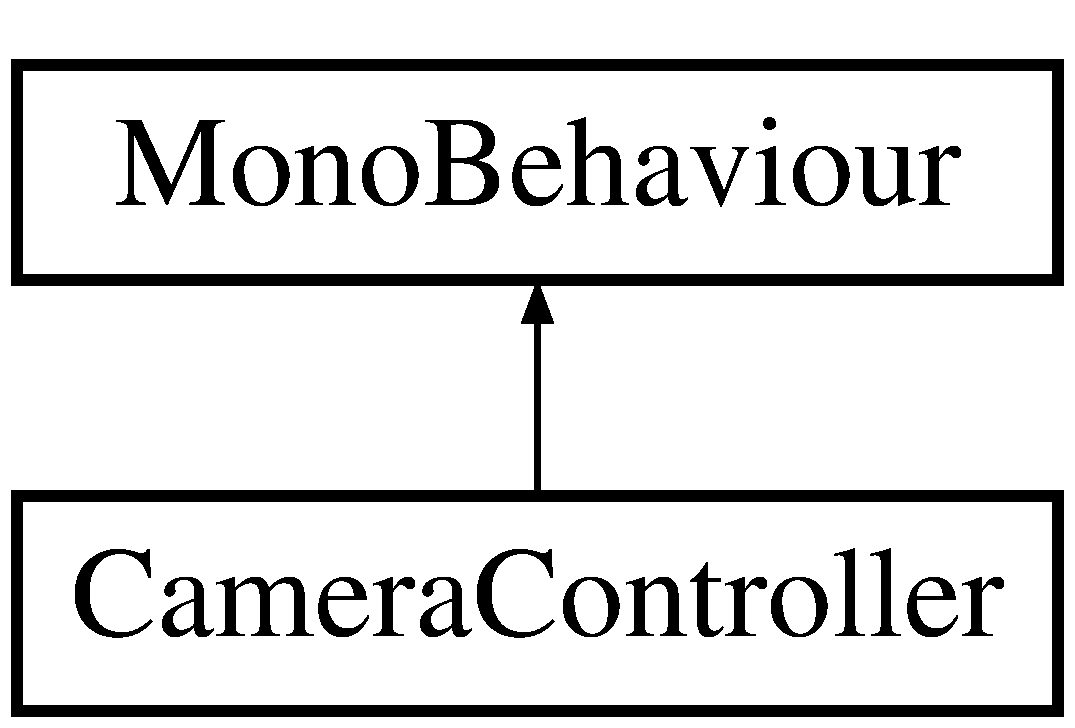
\includegraphics[height=2.000000cm]{class_camera_controller}
\end{center}
\end{figure}
\subsection*{Public Attributes}
\begin{DoxyCompactItemize}
\item 
Game\+Object \mbox{\hyperlink{class_camera_controller_a1bfdfa348a7f9bb2c8d511d9ee3435b9}{follow\+Target}}
\begin{DoxyCompactList}\small\item\em Camera will follow player, create a target position and correlate with a move speed \end{DoxyCompactList}\item 
\mbox{\Hypertarget{class_camera_controller_a8979cceb75638fe3caf62c8516ec4bc6}\label{class_camera_controller_a8979cceb75638fe3caf62c8516ec4bc6}} 
float {\bfseries move\+Speed}
\end{DoxyCompactItemize}
\subsection*{Private Member Functions}
\begin{DoxyCompactItemize}
\item 
void \mbox{\hyperlink{class_camera_controller_ad4a238c6f7db3ee003302a245d860860}{Start}} ()
\begin{DoxyCompactList}\small\item\em Game will not destroy the camera on start If no camera exists, a camera will be made If camera exists, it will be destroyed and a new one will be made \end{DoxyCompactList}\item 
void \mbox{\hyperlink{class_camera_controller_a7c4f486f4bcbd1d54a346fdce9707bd5}{Update}} ()
\begin{DoxyCompactList}\small\item\em Camera will follow target position in the x and y directions The move speed of the camera will be smoothed by deltatime \end{DoxyCompactList}\end{DoxyCompactItemize}
\subsection*{Private Attributes}
\begin{DoxyCompactItemize}
\item 
\mbox{\Hypertarget{class_camera_controller_a2184f9f0312b1966a136d765abcf1a59}\label{class_camera_controller_a2184f9f0312b1966a136d765abcf1a59}} 
Vector3 {\bfseries target\+Pos}
\end{DoxyCompactItemize}
\subsection*{Static Private Attributes}
\begin{DoxyCompactItemize}
\item 
static bool \mbox{\hyperlink{class_camera_controller_a2569b5df8af02ceb1c47be482616b638}{camera\+Exists}}
\begin{DoxyCompactList}\small\item\em Camera either exists or it does not \end{DoxyCompactList}\end{DoxyCompactItemize}


\subsection{Member Function Documentation}
\mbox{\Hypertarget{class_camera_controller_ad4a238c6f7db3ee003302a245d860860}\label{class_camera_controller_ad4a238c6f7db3ee003302a245d860860}} 
\index{Camera\+Controller@{Camera\+Controller}!Start@{Start}}
\index{Start@{Start}!Camera\+Controller@{Camera\+Controller}}
\subsubsection{\texorpdfstring{Start()}{Start()}}
{\footnotesize\ttfamily void Camera\+Controller.\+Start (\begin{DoxyParamCaption}{ }\end{DoxyParamCaption})\hspace{0.3cm}{\ttfamily [private]}}



Game will not destroy the camera on start If no camera exists, a camera will be made If camera exists, it will be destroyed and a new one will be made 

\mbox{\Hypertarget{class_camera_controller_a7c4f486f4bcbd1d54a346fdce9707bd5}\label{class_camera_controller_a7c4f486f4bcbd1d54a346fdce9707bd5}} 
\index{Camera\+Controller@{Camera\+Controller}!Update@{Update}}
\index{Update@{Update}!Camera\+Controller@{Camera\+Controller}}
\subsubsection{\texorpdfstring{Update()}{Update()}}
{\footnotesize\ttfamily void Camera\+Controller.\+Update (\begin{DoxyParamCaption}{ }\end{DoxyParamCaption})\hspace{0.3cm}{\ttfamily [private]}}



Camera will follow target position in the x and y directions The move speed of the camera will be smoothed by deltatime 



\subsection{Member Data Documentation}
\mbox{\Hypertarget{class_camera_controller_a2569b5df8af02ceb1c47be482616b638}\label{class_camera_controller_a2569b5df8af02ceb1c47be482616b638}} 
\index{Camera\+Controller@{Camera\+Controller}!camera\+Exists@{camera\+Exists}}
\index{camera\+Exists@{camera\+Exists}!Camera\+Controller@{Camera\+Controller}}
\subsubsection{\texorpdfstring{camera\+Exists}{cameraExists}}
{\footnotesize\ttfamily bool Camera\+Controller.\+camera\+Exists\hspace{0.3cm}{\ttfamily [static]}, {\ttfamily [private]}}



Camera either exists or it does not 

\mbox{\Hypertarget{class_camera_controller_a1bfdfa348a7f9bb2c8d511d9ee3435b9}\label{class_camera_controller_a1bfdfa348a7f9bb2c8d511d9ee3435b9}} 
\index{Camera\+Controller@{Camera\+Controller}!follow\+Target@{follow\+Target}}
\index{follow\+Target@{follow\+Target}!Camera\+Controller@{Camera\+Controller}}
\subsubsection{\texorpdfstring{follow\+Target}{followTarget}}
{\footnotesize\ttfamily Game\+Object Camera\+Controller.\+follow\+Target}



Camera will follow player, create a target position and correlate with a move speed 



The documentation for this class was generated from the following file\+:\begin{DoxyCompactItemize}
\item 
C\+:/\+Users/\+Am/\+Documents/\+Blue\+Shells -\/ Copy/\+Blue\+Shells/\+Seniors\+Gone\+Wild/\+Assets/\+Scripts/Camera\+Controller.\+cs\end{DoxyCompactItemize}

\hypertarget{class_exit_game}{}\section{Exit\+Game Class Reference}
\label{class_exit_game}\index{Exit\+Game@{Exit\+Game}}
Inheritance diagram for Exit\+Game\+:\begin{figure}[H]
\begin{center}
\leavevmode
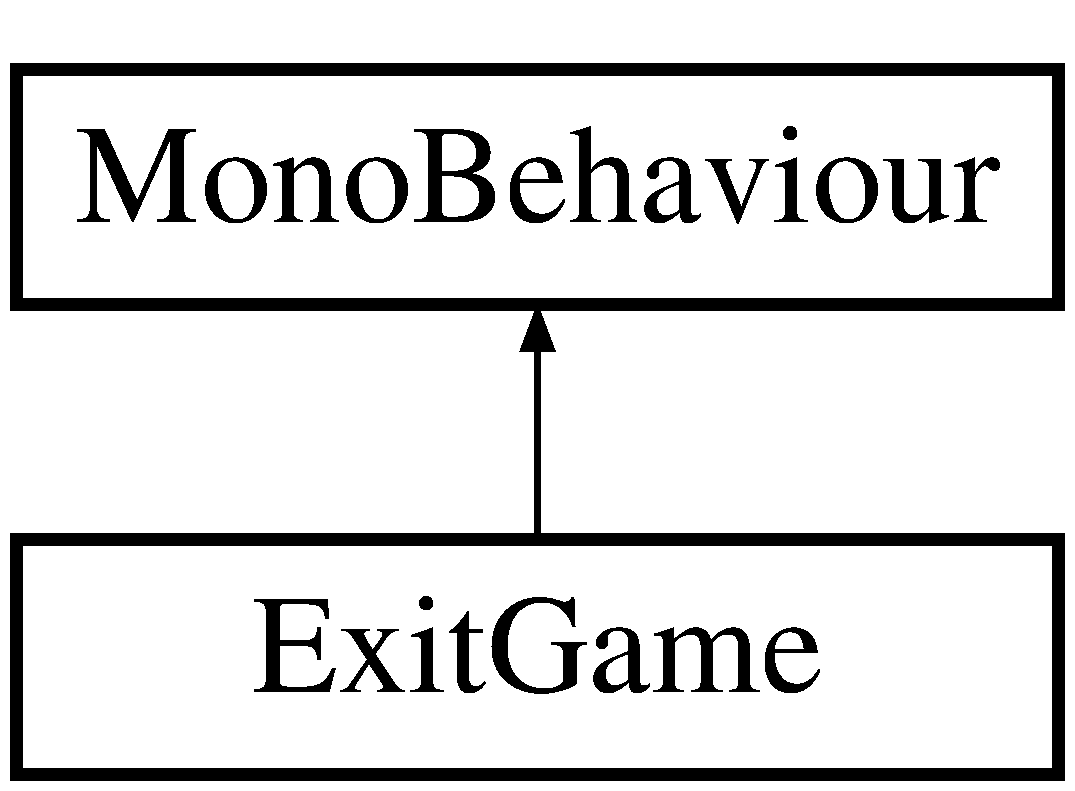
\includegraphics[height=2.000000cm]{class_exit_game}
\end{center}
\end{figure}
\subsection*{Public Attributes}
\begin{DoxyCompactItemize}
\item 
\mbox{\Hypertarget{class_exit_game_ad6440f83b717879b937952479cb993db}\label{class_exit_game_ad6440f83b717879b937952479cb993db}} 
string {\bfseries level\+To\+Load}
\end{DoxyCompactItemize}
\subsection*{Private Member Functions}
\begin{DoxyCompactItemize}
\item 
\mbox{\Hypertarget{class_exit_game_a974a7e22cd4534905c5f3a5bc71b1911}\label{class_exit_game_a974a7e22cd4534905c5f3a5bc71b1911}} 
void {\bfseries Start} ()
\item 
\mbox{\Hypertarget{class_exit_game_aa885bfa25f536f607fea2cb2f5ae487c}\label{class_exit_game_aa885bfa25f536f607fea2cb2f5ae487c}} 
void {\bfseries Update} ()
\item 
void \mbox{\hyperlink{class_exit_game_a8f08c761927046e6e12aad0e76907609}{On\+Trigger\+Enter2D}} (Collider2D other)
\begin{DoxyCompactList}\small\item\em Fucntion used for the final game exit, attached to the final door in the third level If the player reaches the final door, it will load Credits \end{DoxyCompactList}\end{DoxyCompactItemize}


\subsection{Member Function Documentation}
\mbox{\Hypertarget{class_exit_game_a8f08c761927046e6e12aad0e76907609}\label{class_exit_game_a8f08c761927046e6e12aad0e76907609}} 
\index{Exit\+Game@{Exit\+Game}!On\+Trigger\+Enter2D@{On\+Trigger\+Enter2D}}
\index{On\+Trigger\+Enter2D@{On\+Trigger\+Enter2D}!Exit\+Game@{Exit\+Game}}
\subsubsection{\texorpdfstring{On\+Trigger\+Enter2\+D()}{OnTriggerEnter2D()}}
{\footnotesize\ttfamily void Exit\+Game.\+On\+Trigger\+Enter2D (\begin{DoxyParamCaption}\item[{Collider2D}]{other }\end{DoxyParamCaption})\hspace{0.3cm}{\ttfamily [private]}}



Fucntion used for the final game exit, attached to the final door in the third level If the player reaches the final door, it will load Credits 


\begin{DoxyParams}{Parameters}
{\em other} & Other.\\
\hline
\end{DoxyParams}


The documentation for this class was generated from the following file\+:\begin{DoxyCompactItemize}
\item 
C\+:/\+Users/\+Am/\+Documents/\+Blue\+Shells -\/ Copy/\+Blue\+Shells/\+Seniors\+Gone\+Wild/\+Assets/\+Scripts/Exit\+Game.\+cs\end{DoxyCompactItemize}

\hypertarget{class_high_score}{}\section{High\+Score Class Reference}
\label{class_high_score}\index{High\+Score@{High\+Score}}


Creates Score, Name, and ID variables for the database I\+Comparable command used for sorthing the scores  


Inheritance diagram for High\+Score\+:\begin{figure}[H]
\begin{center}
\leavevmode
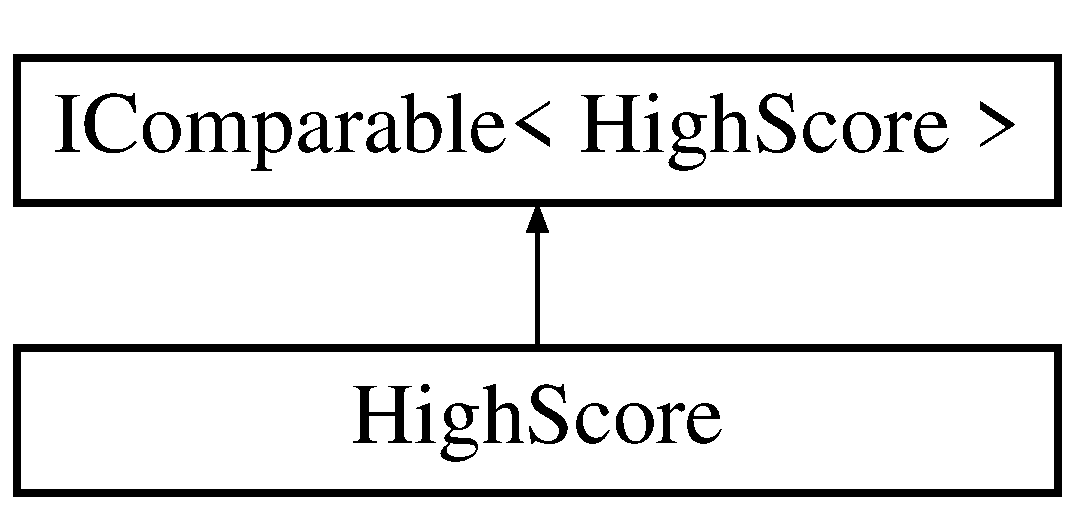
\includegraphics[height=2.000000cm]{class_high_score}
\end{center}
\end{figure}
\subsection*{Public Member Functions}
\begin{DoxyCompactItemize}
\item 
\mbox{\Hypertarget{class_high_score_a5daf0643089c0f0e39a6edfd3e18b56d}\label{class_high_score_a5daf0643089c0f0e39a6edfd3e18b56d}} 
{\bfseries High\+Score} (int id, int score, string name)
\item 
int \mbox{\hyperlink{class_high_score_acd16825af79f7d613806515c82d27674}{Compare\+To}} (\mbox{\hyperlink{class_high_score}{High\+Score}} other)
\begin{DoxyCompactList}\small\item\em Function used to compare the scores in order to sort and delete later on first $>$ second return -\/1 first $<$ second return 1 first == second return 0 \end{DoxyCompactList}\end{DoxyCompactItemize}
\subsection*{Properties}
\begin{DoxyCompactItemize}
\item 
\mbox{\Hypertarget{class_high_score_a3f5ecd5b588c553ac2f35fb25cd7cbda}\label{class_high_score_a3f5ecd5b588c553ac2f35fb25cd7cbda}} 
int {\bfseries Score}\hspace{0.3cm}{\ttfamily  \mbox{[}get, set\mbox{]}}
\item 
\mbox{\Hypertarget{class_high_score_a60bfe5afabcb76145a58093d8d2c415c}\label{class_high_score_a60bfe5afabcb76145a58093d8d2c415c}} 
string {\bfseries Name}\hspace{0.3cm}{\ttfamily  \mbox{[}get, set\mbox{]}}
\item 
\mbox{\Hypertarget{class_high_score_a8847e1da15aec2b4b3848fdf8ee5eabf}\label{class_high_score_a8847e1da15aec2b4b3848fdf8ee5eabf}} 
int {\bfseries ID}\hspace{0.3cm}{\ttfamily  \mbox{[}get, set\mbox{]}}
\end{DoxyCompactItemize}


\subsection{Detailed Description}
Creates Score, Name, and ID variables for the database I\+Comparable command used for sorthing the scores 

The score.

\subsection{Member Function Documentation}
\mbox{\Hypertarget{class_high_score_acd16825af79f7d613806515c82d27674}\label{class_high_score_acd16825af79f7d613806515c82d27674}} 
\index{High\+Score@{High\+Score}!Compare\+To@{Compare\+To}}
\index{Compare\+To@{Compare\+To}!High\+Score@{High\+Score}}
\subsubsection{\texorpdfstring{Compare\+To()}{CompareTo()}}
{\footnotesize\ttfamily int High\+Score.\+Compare\+To (\begin{DoxyParamCaption}\item[{\mbox{\hyperlink{class_high_score}{High\+Score}}}]{other }\end{DoxyParamCaption})}



Function used to compare the scores in order to sort and delete later on first $>$ second return -\/1 first $<$ second return 1 first == second return 0 

\begin{DoxyReturn}{Returns}
The to.
\end{DoxyReturn}

\begin{DoxyParams}{Parameters}
{\em other} & Other.\\
\hline
\end{DoxyParams}


The documentation for this class was generated from the following file\+:\begin{DoxyCompactItemize}
\item 
C\+:/\+Users/\+Am/\+Documents/\+Blue\+Shells -\/ Copy/\+Blue\+Shells/\+Seniors\+Gone\+Wild/\+Assets/\+Scripts/High\+Score.\+cs\end{DoxyCompactItemize}

\hypertarget{class_high_score_manager}{}\section{High\+Score\+Manager Class Reference}
\label{class_high_score_manager}\index{High\+Score\+Manager@{High\+Score\+Manager}}
Inheritance diagram for High\+Score\+Manager\+:\begin{figure}[H]
\begin{center}
\leavevmode
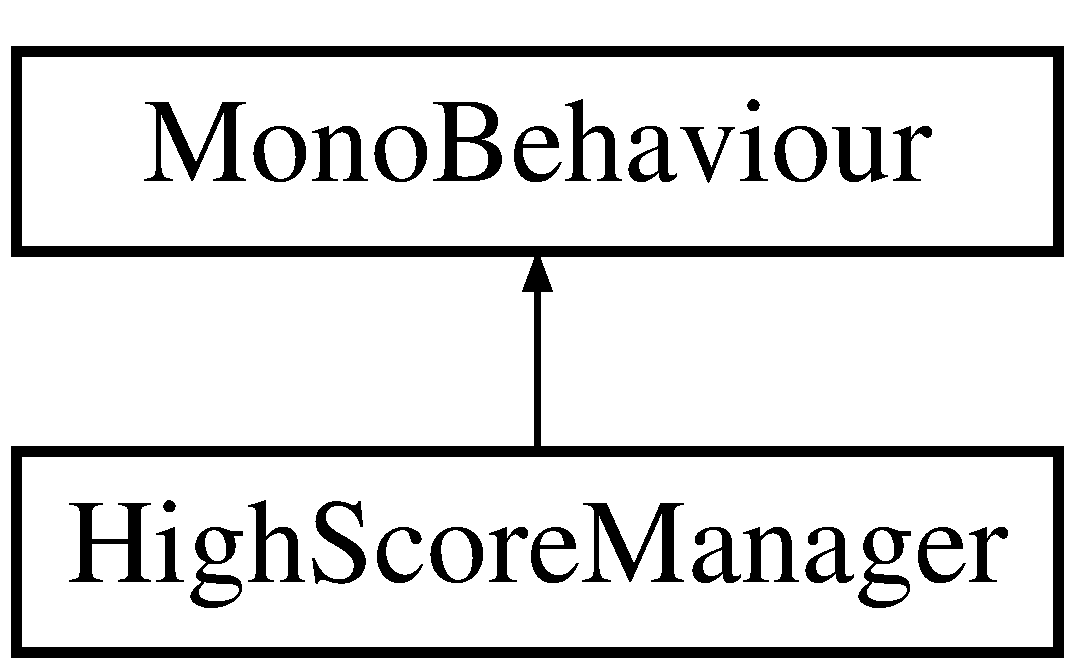
\includegraphics[height=2.000000cm]{class_high_score_manager}
\end{center}
\end{figure}
\subsection*{Public Member Functions}
\begin{DoxyCompactItemize}
\item 
void \mbox{\hyperlink{class_high_score_manager_a098d1e52bc63ab8c014fa1210d04481e}{Enter\+Name}} ()
\begin{DoxyCompactList}\small\item\em This function checks if the player has entered a name or not It sets the player\textquotesingle{}s score, taken from the \mbox{\hyperlink{class_nurse_controller}{Nurse\+Controller}} It will then enter the name, and show the previous scores \end{DoxyCompactList}\end{DoxyCompactItemize}
\subsection*{Public Attributes}
\begin{DoxyCompactItemize}
\item 
\mbox{\Hypertarget{class_high_score_manager_ac7fb552c1ee9bf4415e74adfa005a103}\label{class_high_score_manager_ac7fb552c1ee9bf4415e74adfa005a103}} 
Game\+Object {\bfseries score\+Prefab}
\item 
\mbox{\Hypertarget{class_high_score_manager_ae76705d7b8e7717f09dcb7b6950cd327}\label{class_high_score_manager_ae76705d7b8e7717f09dcb7b6950cd327}} 
Game\+Object {\bfseries name\+Dialog}
\item 
\mbox{\Hypertarget{class_high_score_manager_a8fc762843b986cf1bf477f78e4685761}\label{class_high_score_manager_a8fc762843b986cf1bf477f78e4685761}} 
Transform {\bfseries score\+Parent}
\item 
\mbox{\Hypertarget{class_high_score_manager_a331c0091b70ade22473e2ea320cb2ce7}\label{class_high_score_manager_a331c0091b70ade22473e2ea320cb2ce7}} 
int {\bfseries top\+Ranks}
\item 
\mbox{\Hypertarget{class_high_score_manager_a22c1d47f968a21f33e253b94657ae773}\label{class_high_score_manager_a22c1d47f968a21f33e253b94657ae773}} 
int {\bfseries save\+Scores}
\item 
\mbox{\Hypertarget{class_high_score_manager_ae186979c1ae3245b63d05fd2f315788d}\label{class_high_score_manager_ae186979c1ae3245b63d05fd2f315788d}} 
Input\+Field {\bfseries enter\+Name}
\end{DoxyCompactItemize}
\subsection*{Private Member Functions}
\begin{DoxyCompactItemize}
\item 
void \mbox{\hyperlink{class_high_score_manager_acee896a71e1b9f5bb9c486d373331df0}{Start}} ()
\begin{DoxyCompactList}\small\item\em The start contains all of the functions we will use to update the high score list This sets a path that goes directly to the database created for the game \end{DoxyCompactList}\item 
void \mbox{\hyperlink{class_high_score_manager_ad75f6456ad76309b4744a3c592da7443}{Update}} ()
\begin{DoxyCompactList}\small\item\em This is used for the \char`\"{}\+Insert Name\char`\"{} box It is activated upon using the escape key \end{DoxyCompactList}\item 
void \mbox{\hyperlink{class_high_score_manager_a4a5a8e7cf5168aba0841c78432294a4a}{Create\+Table}} ()
\begin{DoxyCompactList}\small\item\em This function creates the database table inside the C\# and unity files \end{DoxyCompactList}\item 
void \mbox{\hyperlink{class_high_score_manager_a45ea58b135c4050aedaad4e12ffadbe3}{Insert\+Score}} (string name, int new\+Score)
\begin{DoxyCompactList}\small\item\em This function compares the scores and adjusts the rankings. Our scoreboard shows the top 10, so it removes the lowest score instead of the highest It opens and closes the connection to the database via S\+QL queries \end{DoxyCompactList}\item 
void \mbox{\hyperlink{class_high_score_manager_ac0ebc45a4af433ca6f19c06096bd072f}{Get\+Scores}} ()
\begin{DoxyCompactList}\small\item\em This function retrieves the scores from the database and inserts them into the unity scoreboard and then sorts them in highest-\/lowest order \end{DoxyCompactList}\item 
void \mbox{\hyperlink{class_high_score_manager_a2051e83d70923629fdc6bd68c7e4eac9}{Delete\+Score}} (int id)
\begin{DoxyCompactList}\small\item\em This function is called upon to delete a score when a newer, higher score is inserted into the database, thus taking it off the high score list \end{DoxyCompactList}\item 
void \mbox{\hyperlink{class_high_score_manager_ab3e52344cd580a8e4e68f741361072e4}{Show\+Scores}} ()
\begin{DoxyCompactList}\small\item\em This function is used to destroy all of the scores, in order to reinsert them into the database to ensure that no repeats are made It changes the scoreboard information, and inserts a \char`\"{}\#\char`\"{} before the rank It also includes \char`\"{}i + 1\char`\"{} which starts the ranks from 1 instead of 0 It includes organizational elements such as the prefab and parent items which is where the scores are inserted \end{DoxyCompactList}\item 
void \mbox{\hyperlink{class_high_score_manager_a6b8807e7293dddf882b3faf180e68ecd}{Delete\+Extra\+Score}} ()
\begin{DoxyCompactList}\small\item\em Deletes extra scores from the database based on our limit \end{DoxyCompactList}\end{DoxyCompactItemize}
\subsection*{Private Attributes}
\begin{DoxyCompactItemize}
\item 
string \mbox{\hyperlink{class_high_score_manager_a9d8d74d89d2986ad69f282c1129d04a9}{connection\+String}}
\begin{DoxyCompactList}\small\item\em All variables are elements used for the format of the high score appearance \end{DoxyCompactList}\item 
\mbox{\Hypertarget{class_high_score_manager_a9fa93771421f2616616eb71cd1e6ec2d}\label{class_high_score_manager_a9fa93771421f2616616eb71cd1e6ec2d}} 
List$<$ \mbox{\hyperlink{class_high_score}{High\+Score}} $>$ {\bfseries high\+Scores} = new List$<$\mbox{\hyperlink{class_high_score}{High\+Score}}$>$ ()
\end{DoxyCompactItemize}


\subsection{Member Function Documentation}
\mbox{\Hypertarget{class_high_score_manager_a4a5a8e7cf5168aba0841c78432294a4a}\label{class_high_score_manager_a4a5a8e7cf5168aba0841c78432294a4a}} 
\index{High\+Score\+Manager@{High\+Score\+Manager}!Create\+Table@{Create\+Table}}
\index{Create\+Table@{Create\+Table}!High\+Score\+Manager@{High\+Score\+Manager}}
\subsubsection{\texorpdfstring{Create\+Table()}{CreateTable()}}
{\footnotesize\ttfamily void High\+Score\+Manager.\+Create\+Table (\begin{DoxyParamCaption}{ }\end{DoxyParamCaption})\hspace{0.3cm}{\ttfamily [private]}}



This function creates the database table inside the C\# and unity files 

\mbox{\Hypertarget{class_high_score_manager_a6b8807e7293dddf882b3faf180e68ecd}\label{class_high_score_manager_a6b8807e7293dddf882b3faf180e68ecd}} 
\index{High\+Score\+Manager@{High\+Score\+Manager}!Delete\+Extra\+Score@{Delete\+Extra\+Score}}
\index{Delete\+Extra\+Score@{Delete\+Extra\+Score}!High\+Score\+Manager@{High\+Score\+Manager}}
\subsubsection{\texorpdfstring{Delete\+Extra\+Score()}{DeleteExtraScore()}}
{\footnotesize\ttfamily void High\+Score\+Manager.\+Delete\+Extra\+Score (\begin{DoxyParamCaption}{ }\end{DoxyParamCaption})\hspace{0.3cm}{\ttfamily [private]}}



Deletes extra scores from the database based on our limit 

\mbox{\Hypertarget{class_high_score_manager_a2051e83d70923629fdc6bd68c7e4eac9}\label{class_high_score_manager_a2051e83d70923629fdc6bd68c7e4eac9}} 
\index{High\+Score\+Manager@{High\+Score\+Manager}!Delete\+Score@{Delete\+Score}}
\index{Delete\+Score@{Delete\+Score}!High\+Score\+Manager@{High\+Score\+Manager}}
\subsubsection{\texorpdfstring{Delete\+Score()}{DeleteScore()}}
{\footnotesize\ttfamily void High\+Score\+Manager.\+Delete\+Score (\begin{DoxyParamCaption}\item[{int}]{id }\end{DoxyParamCaption})\hspace{0.3cm}{\ttfamily [private]}}



This function is called upon to delete a score when a newer, higher score is inserted into the database, thus taking it off the high score list 


\begin{DoxyParams}{Parameters}
{\em id} & Identifier.\\
\hline
\end{DoxyParams}
\mbox{\Hypertarget{class_high_score_manager_a098d1e52bc63ab8c014fa1210d04481e}\label{class_high_score_manager_a098d1e52bc63ab8c014fa1210d04481e}} 
\index{High\+Score\+Manager@{High\+Score\+Manager}!Enter\+Name@{Enter\+Name}}
\index{Enter\+Name@{Enter\+Name}!High\+Score\+Manager@{High\+Score\+Manager}}
\subsubsection{\texorpdfstring{Enter\+Name()}{EnterName()}}
{\footnotesize\ttfamily void High\+Score\+Manager.\+Enter\+Name (\begin{DoxyParamCaption}{ }\end{DoxyParamCaption})}



This function checks if the player has entered a name or not It sets the player\textquotesingle{}s score, taken from the \mbox{\hyperlink{class_nurse_controller}{Nurse\+Controller}} It will then enter the name, and show the previous scores 

\mbox{\Hypertarget{class_high_score_manager_ac0ebc45a4af433ca6f19c06096bd072f}\label{class_high_score_manager_ac0ebc45a4af433ca6f19c06096bd072f}} 
\index{High\+Score\+Manager@{High\+Score\+Manager}!Get\+Scores@{Get\+Scores}}
\index{Get\+Scores@{Get\+Scores}!High\+Score\+Manager@{High\+Score\+Manager}}
\subsubsection{\texorpdfstring{Get\+Scores()}{GetScores()}}
{\footnotesize\ttfamily void High\+Score\+Manager.\+Get\+Scores (\begin{DoxyParamCaption}{ }\end{DoxyParamCaption})\hspace{0.3cm}{\ttfamily [private]}}



This function retrieves the scores from the database and inserts them into the unity scoreboard and then sorts them in highest-\/lowest order 

\mbox{\Hypertarget{class_high_score_manager_a45ea58b135c4050aedaad4e12ffadbe3}\label{class_high_score_manager_a45ea58b135c4050aedaad4e12ffadbe3}} 
\index{High\+Score\+Manager@{High\+Score\+Manager}!Insert\+Score@{Insert\+Score}}
\index{Insert\+Score@{Insert\+Score}!High\+Score\+Manager@{High\+Score\+Manager}}
\subsubsection{\texorpdfstring{Insert\+Score()}{InsertScore()}}
{\footnotesize\ttfamily void High\+Score\+Manager.\+Insert\+Score (\begin{DoxyParamCaption}\item[{string}]{name,  }\item[{int}]{new\+Score }\end{DoxyParamCaption})\hspace{0.3cm}{\ttfamily [private]}}



This function compares the scores and adjusts the rankings. Our scoreboard shows the top 10, so it removes the lowest score instead of the highest It opens and closes the connection to the database via S\+QL queries 


\begin{DoxyParams}{Parameters}
{\em name} & Name.\\
\hline
{\em new\+Score} & New score.\\
\hline
\end{DoxyParams}
\mbox{\Hypertarget{class_high_score_manager_ab3e52344cd580a8e4e68f741361072e4}\label{class_high_score_manager_ab3e52344cd580a8e4e68f741361072e4}} 
\index{High\+Score\+Manager@{High\+Score\+Manager}!Show\+Scores@{Show\+Scores}}
\index{Show\+Scores@{Show\+Scores}!High\+Score\+Manager@{High\+Score\+Manager}}
\subsubsection{\texorpdfstring{Show\+Scores()}{ShowScores()}}
{\footnotesize\ttfamily void High\+Score\+Manager.\+Show\+Scores (\begin{DoxyParamCaption}{ }\end{DoxyParamCaption})\hspace{0.3cm}{\ttfamily [private]}}



This function is used to destroy all of the scores, in order to reinsert them into the database to ensure that no repeats are made It changes the scoreboard information, and inserts a \char`\"{}\#\char`\"{} before the rank It also includes \char`\"{}i + 1\char`\"{} which starts the ranks from 1 instead of 0 It includes organizational elements such as the prefab and parent items which is where the scores are inserted 

\mbox{\Hypertarget{class_high_score_manager_acee896a71e1b9f5bb9c486d373331df0}\label{class_high_score_manager_acee896a71e1b9f5bb9c486d373331df0}} 
\index{High\+Score\+Manager@{High\+Score\+Manager}!Start@{Start}}
\index{Start@{Start}!High\+Score\+Manager@{High\+Score\+Manager}}
\subsubsection{\texorpdfstring{Start()}{Start()}}
{\footnotesize\ttfamily void High\+Score\+Manager.\+Start (\begin{DoxyParamCaption}{ }\end{DoxyParamCaption})\hspace{0.3cm}{\ttfamily [private]}}



The start contains all of the functions we will use to update the high score list This sets a path that goes directly to the database created for the game 

\mbox{\Hypertarget{class_high_score_manager_ad75f6456ad76309b4744a3c592da7443}\label{class_high_score_manager_ad75f6456ad76309b4744a3c592da7443}} 
\index{High\+Score\+Manager@{High\+Score\+Manager}!Update@{Update}}
\index{Update@{Update}!High\+Score\+Manager@{High\+Score\+Manager}}
\subsubsection{\texorpdfstring{Update()}{Update()}}
{\footnotesize\ttfamily void High\+Score\+Manager.\+Update (\begin{DoxyParamCaption}{ }\end{DoxyParamCaption})\hspace{0.3cm}{\ttfamily [private]}}



This is used for the \char`\"{}\+Insert Name\char`\"{} box It is activated upon using the escape key 



\subsection{Member Data Documentation}
\mbox{\Hypertarget{class_high_score_manager_a9d8d74d89d2986ad69f282c1129d04a9}\label{class_high_score_manager_a9d8d74d89d2986ad69f282c1129d04a9}} 
\index{High\+Score\+Manager@{High\+Score\+Manager}!connection\+String@{connection\+String}}
\index{connection\+String@{connection\+String}!High\+Score\+Manager@{High\+Score\+Manager}}
\subsubsection{\texorpdfstring{connection\+String}{connectionString}}
{\footnotesize\ttfamily string High\+Score\+Manager.\+connection\+String\hspace{0.3cm}{\ttfamily [private]}}



All variables are elements used for the format of the high score appearance 



The documentation for this class was generated from the following file\+:\begin{DoxyCompactItemize}
\item 
C\+:/\+Users/\+Am/\+Documents/\+Blue\+Shells -\/ Copy/\+Blue\+Shells/\+Seniors\+Gone\+Wild/\+Assets/\+Scripts/High\+Score\+Manager.\+cs\end{DoxyCompactItemize}

\hypertarget{class_high_score_script}{}\section{High\+Score\+Script Class Reference}
\label{class_high_score_script}\index{High\+Score\+Script@{High\+Score\+Script}}


This script controls the scoreboard and adds information to it. (Like Player name, rank and score)  


Inheritance diagram for High\+Score\+Script\+:\begin{figure}[H]
\begin{center}
\leavevmode
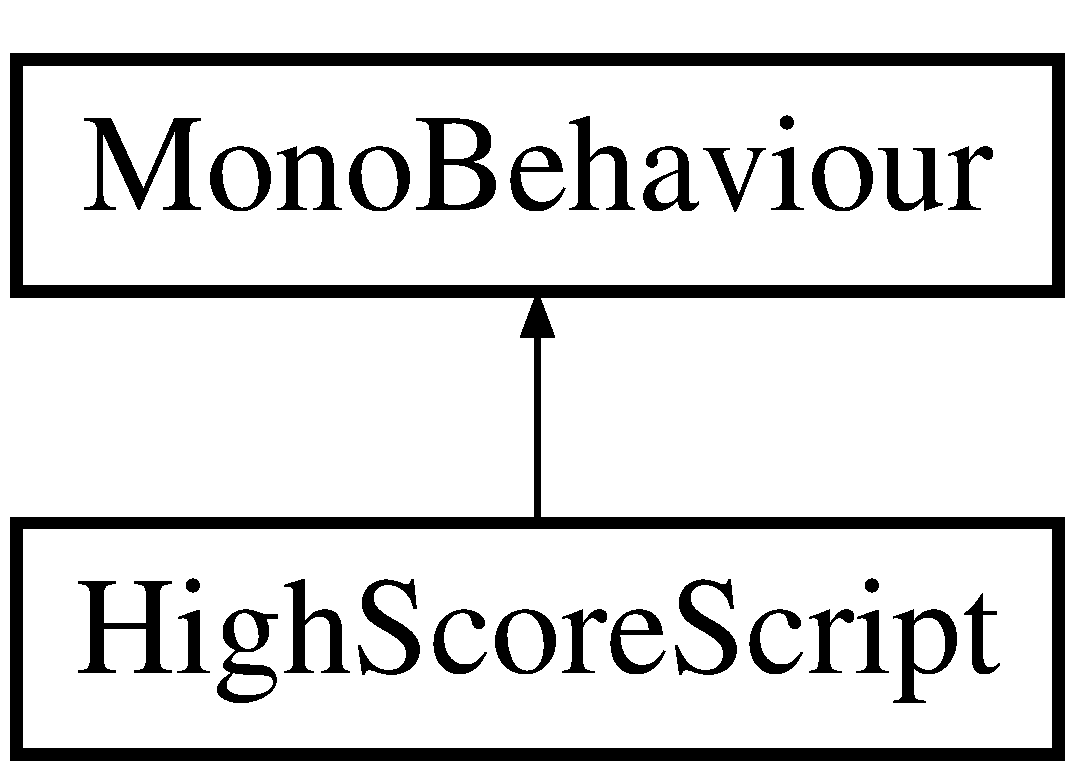
\includegraphics[height=2.000000cm]{class_high_score_script}
\end{center}
\end{figure}
\subsection*{Public Member Functions}
\begin{DoxyCompactItemize}
\item 
void \mbox{\hyperlink{class_high_score_script_ad9ef406b6e411f1a155be9cad38471be}{Set\+Score}} (string name, string \mbox{\hyperlink{class_high_score_script_acaef3205159e2e692bcb140618f2d84d}{score}}, string rank)
\begin{DoxyCompactList}\small\item\em This fucntion modifies the text component and adds text into it \end{DoxyCompactList}\end{DoxyCompactItemize}
\subsection*{Public Attributes}
\begin{DoxyCompactItemize}
\item 
Game\+Object \mbox{\hyperlink{class_high_score_script_acaef3205159e2e692bcb140618f2d84d}{score}}
\begin{DoxyCompactList}\small\item\em Creates score, name and rank variables for the High Score Database \end{DoxyCompactList}\item 
\mbox{\Hypertarget{class_high_score_script_ab62d166f25519842ce8cf7f3f7dbb1ea}\label{class_high_score_script_ab62d166f25519842ce8cf7f3f7dbb1ea}} 
Game\+Object {\bfseries score\+Name}
\item 
\mbox{\Hypertarget{class_high_score_script_a94557499a852364672bda2aec16e2e54}\label{class_high_score_script_a94557499a852364672bda2aec16e2e54}} 
Game\+Object {\bfseries rank}
\end{DoxyCompactItemize}


\subsection{Detailed Description}
This script controls the scoreboard and adds information to it. (Like Player name, rank and score) 



\subsection{Member Function Documentation}
\mbox{\Hypertarget{class_high_score_script_ad9ef406b6e411f1a155be9cad38471be}\label{class_high_score_script_ad9ef406b6e411f1a155be9cad38471be}} 
\index{High\+Score\+Script@{High\+Score\+Script}!Set\+Score@{Set\+Score}}
\index{Set\+Score@{Set\+Score}!High\+Score\+Script@{High\+Score\+Script}}
\subsubsection{\texorpdfstring{Set\+Score()}{SetScore()}}
{\footnotesize\ttfamily void High\+Score\+Script.\+Set\+Score (\begin{DoxyParamCaption}\item[{string}]{name,  }\item[{string}]{score,  }\item[{string}]{rank }\end{DoxyParamCaption})}



This fucntion modifies the text component and adds text into it 


\begin{DoxyParams}{Parameters}
{\em name} & Name.\\
\hline
{\em score} & Score.\\
\hline
{\em rank} & Rank.\\
\hline
\end{DoxyParams}


\subsection{Member Data Documentation}
\mbox{\Hypertarget{class_high_score_script_acaef3205159e2e692bcb140618f2d84d}\label{class_high_score_script_acaef3205159e2e692bcb140618f2d84d}} 
\index{High\+Score\+Script@{High\+Score\+Script}!score@{score}}
\index{score@{score}!High\+Score\+Script@{High\+Score\+Script}}
\subsubsection{\texorpdfstring{score}{score}}
{\footnotesize\ttfamily Game\+Object High\+Score\+Script.\+score}



Creates score, name and rank variables for the High Score Database 



The documentation for this class was generated from the following file\+:\begin{DoxyCompactItemize}
\item 
C\+:/\+Users/\+Am/\+Documents/\+Blue\+Shells -\/ Copy/\+Blue\+Shells/\+Seniors\+Gone\+Wild/\+Assets/\+Scripts/High\+Score\+Script.\+cs\end{DoxyCompactItemize}

\hypertarget{class_load_credits}{}\section{Load\+Credits Class Reference}
\label{class_load_credits}\index{Load\+Credits@{Load\+Credits}}
Inheritance diagram for Load\+Credits\+:\begin{figure}[H]
\begin{center}
\leavevmode
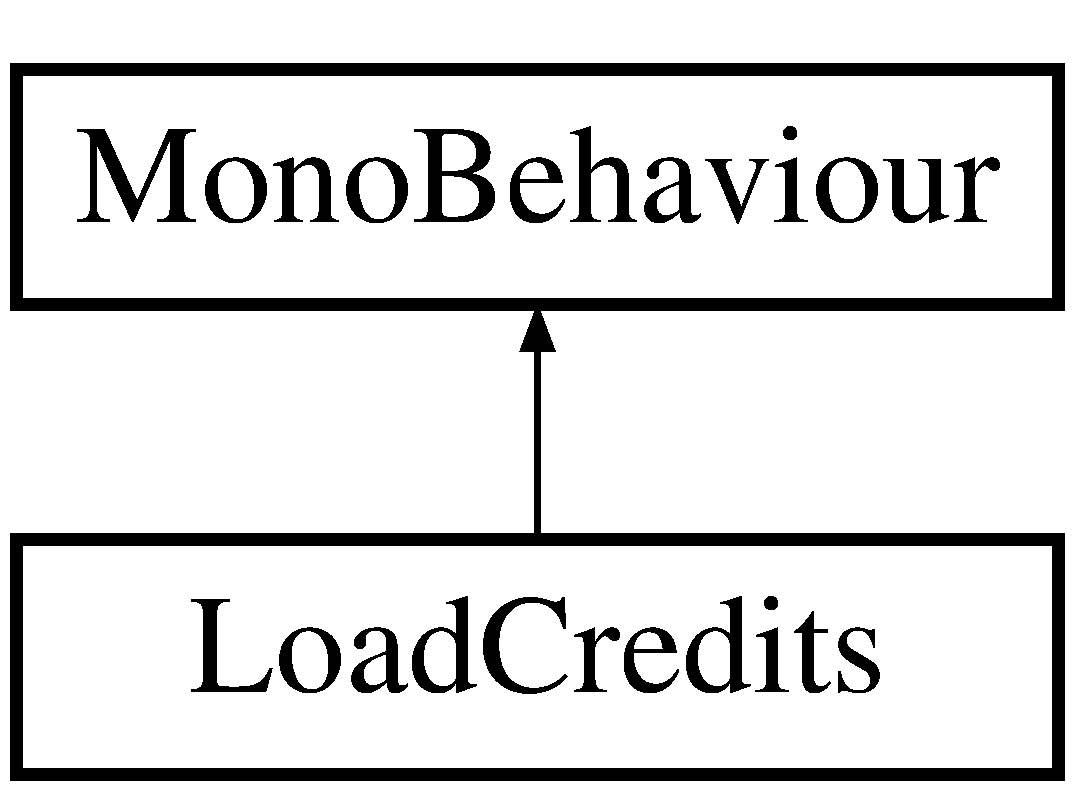
\includegraphics[height=2.000000cm]{class_load_credits}
\end{center}
\end{figure}
\subsection*{Public Member Functions}
\begin{DoxyCompactItemize}
\item 
void \mbox{\hyperlink{class_load_credits_a5a96d132e7cdd4240bb6c596a2e6b3dd}{Load\+Credit}} ()
\begin{DoxyCompactList}\small\item\em This function loads the menu from the End Scene \end{DoxyCompactList}\end{DoxyCompactItemize}


\subsection{Member Function Documentation}
\mbox{\Hypertarget{class_load_credits_a5a96d132e7cdd4240bb6c596a2e6b3dd}\label{class_load_credits_a5a96d132e7cdd4240bb6c596a2e6b3dd}} 
\index{Load\+Credits@{Load\+Credits}!Load\+Credit@{Load\+Credit}}
\index{Load\+Credit@{Load\+Credit}!Load\+Credits@{Load\+Credits}}
\subsubsection{\texorpdfstring{Load\+Credit()}{LoadCredit()}}
{\footnotesize\ttfamily void Load\+Credits.\+Load\+Credit (\begin{DoxyParamCaption}{ }\end{DoxyParamCaption})}



This function loads the menu from the End Scene 



The documentation for this class was generated from the following file\+:\begin{DoxyCompactItemize}
\item 
C\+:/\+Users/\+Am/\+Documents/\+Blue\+Shells -\/ Copy/\+Blue\+Shells/\+Seniors\+Gone\+Wild/\+Assets/\+Scripts/Load\+Credits.\+cs\end{DoxyCompactItemize}

\hypertarget{class_load_escape_scene}{}\section{Load\+Escape\+Scene Class Reference}
\label{class_load_escape_scene}\index{Load\+Escape\+Scene@{Load\+Escape\+Scene}}
Inheritance diagram for Load\+Escape\+Scene\+:\begin{figure}[H]
\begin{center}
\leavevmode
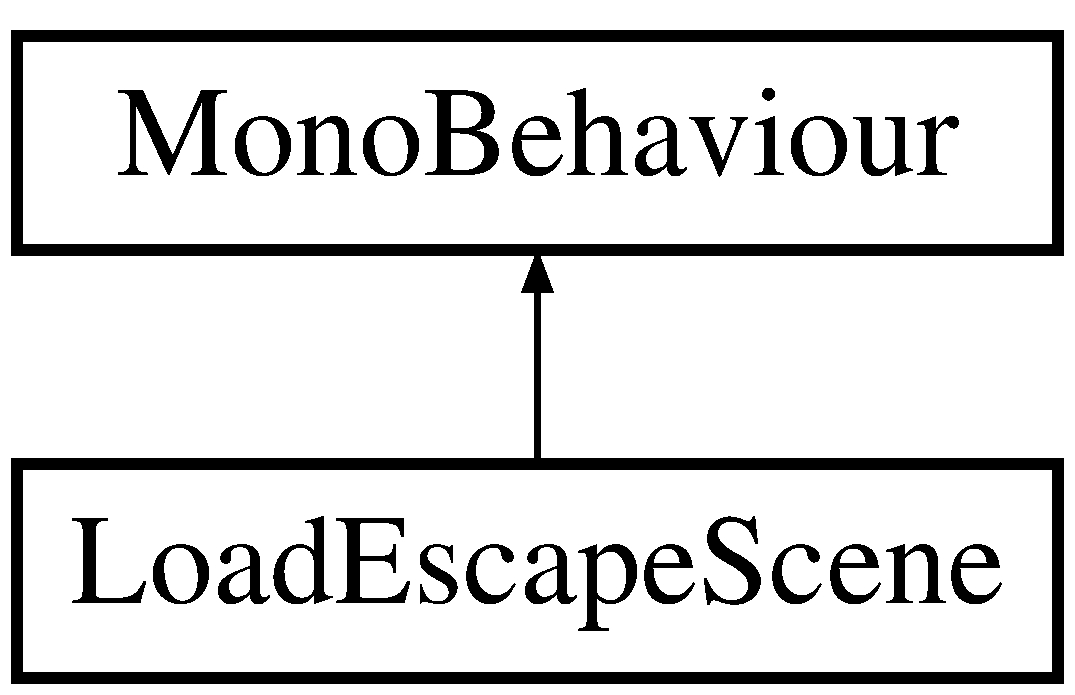
\includegraphics[height=2.000000cm]{class_load_escape_scene}
\end{center}
\end{figure}
\subsection*{Public Attributes}
\begin{DoxyCompactItemize}
\item 
\mbox{\Hypertarget{class_load_escape_scene_a15d6dcb5e40c53c17e2dc7c2fa7319fb}\label{class_load_escape_scene_a15d6dcb5e40c53c17e2dc7c2fa7319fb}} 
string {\bfseries level\+To\+Load}
\end{DoxyCompactItemize}
\subsection*{Private Member Functions}
\begin{DoxyCompactItemize}
\item 
\mbox{\Hypertarget{class_load_escape_scene_a61cdb35e4c56deee7597df7aa16f2877}\label{class_load_escape_scene_a61cdb35e4c56deee7597df7aa16f2877}} 
void {\bfseries Start} ()
\item 
\mbox{\Hypertarget{class_load_escape_scene_ab7580e84f80f4a3c8b390bf113b82761}\label{class_load_escape_scene_ab7580e84f80f4a3c8b390bf113b82761}} 
void {\bfseries Update} ()
\item 
void \mbox{\hyperlink{class_load_escape_scene_a5fd7bb04123701797923ddee003e3ace}{On\+Trigger\+Enter2D}} (Collider2D other)
\begin{DoxyCompactList}\small\item\em This function allows the player to go to the Escape Scene after exiting the final door on the third level The second loop makes sure that the item\+Count resets for the next player \end{DoxyCompactList}\end{DoxyCompactItemize}


\subsection{Member Function Documentation}
\mbox{\Hypertarget{class_load_escape_scene_a5fd7bb04123701797923ddee003e3ace}\label{class_load_escape_scene_a5fd7bb04123701797923ddee003e3ace}} 
\index{Load\+Escape\+Scene@{Load\+Escape\+Scene}!On\+Trigger\+Enter2D@{On\+Trigger\+Enter2D}}
\index{On\+Trigger\+Enter2D@{On\+Trigger\+Enter2D}!Load\+Escape\+Scene@{Load\+Escape\+Scene}}
\subsubsection{\texorpdfstring{On\+Trigger\+Enter2\+D()}{OnTriggerEnter2D()}}
{\footnotesize\ttfamily void Load\+Escape\+Scene.\+On\+Trigger\+Enter2D (\begin{DoxyParamCaption}\item[{Collider2D}]{other }\end{DoxyParamCaption})\hspace{0.3cm}{\ttfamily [private]}}



This function allows the player to go to the Escape Scene after exiting the final door on the third level The second loop makes sure that the item\+Count resets for the next player 


\begin{DoxyParams}{Parameters}
{\em other} & Other.\\
\hline
\end{DoxyParams}


The documentation for this class was generated from the following file\+:\begin{DoxyCompactItemize}
\item 
C\+:/\+Users/\+Am/\+Documents/\+Blue\+Shells -\/ Copy/\+Blue\+Shells/\+Seniors\+Gone\+Wild/\+Assets/\+Scripts/Load\+Escape\+Scene.\+cs\end{DoxyCompactItemize}

\hypertarget{class_load_high_scores}{}\section{Load\+High\+Scores Class Reference}
\label{class_load_high_scores}\index{Load\+High\+Scores@{Load\+High\+Scores}}
Inheritance diagram for Load\+High\+Scores\+:\begin{figure}[H]
\begin{center}
\leavevmode
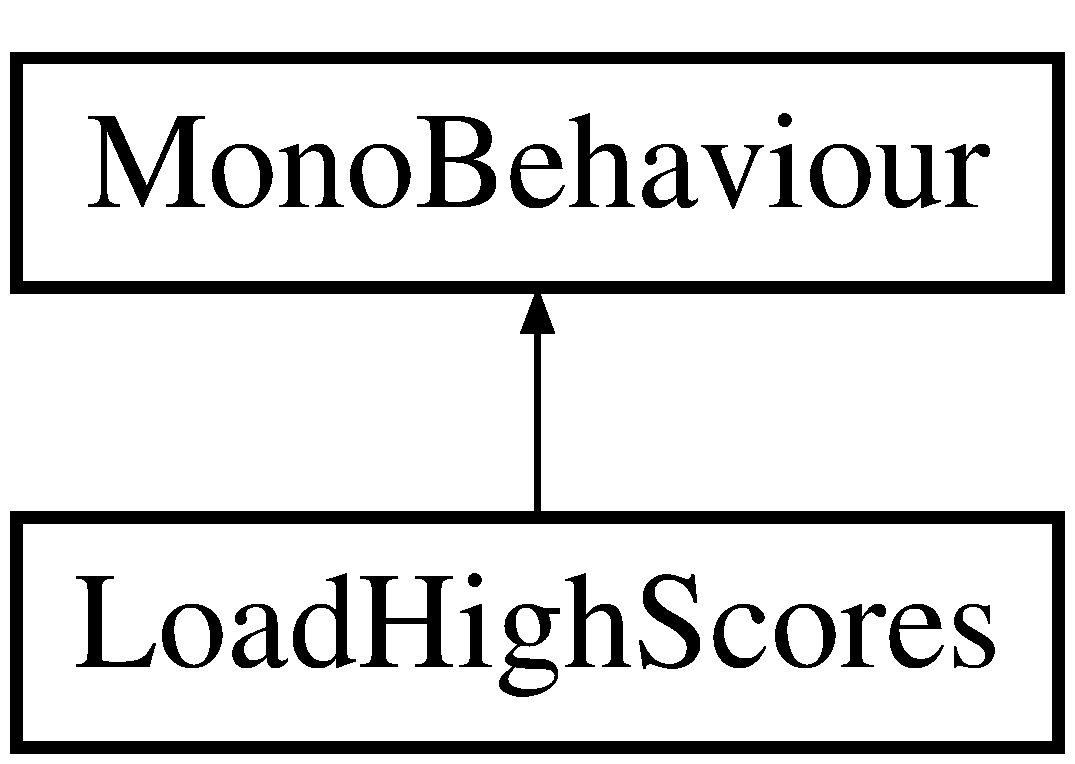
\includegraphics[height=2.000000cm]{class_load_high_scores}
\end{center}
\end{figure}
\subsection*{Public Member Functions}
\begin{DoxyCompactItemize}
\item 
void \mbox{\hyperlink{class_load_high_scores_a70d2922d1154abdd92e247e3ea9f11e5}{Load\+End\+Scene}} ()
\begin{DoxyCompactList}\small\item\em This function loads the End\+Scene from the credits page \end{DoxyCompactList}\end{DoxyCompactItemize}


\subsection{Member Function Documentation}
\mbox{\Hypertarget{class_load_high_scores_a70d2922d1154abdd92e247e3ea9f11e5}\label{class_load_high_scores_a70d2922d1154abdd92e247e3ea9f11e5}} 
\index{Load\+High\+Scores@{Load\+High\+Scores}!Load\+End\+Scene@{Load\+End\+Scene}}
\index{Load\+End\+Scene@{Load\+End\+Scene}!Load\+High\+Scores@{Load\+High\+Scores}}
\subsubsection{\texorpdfstring{Load\+End\+Scene()}{LoadEndScene()}}
{\footnotesize\ttfamily void Load\+High\+Scores.\+Load\+End\+Scene (\begin{DoxyParamCaption}{ }\end{DoxyParamCaption})}



This function loads the End\+Scene from the credits page 



The documentation for this class was generated from the following file\+:\begin{DoxyCompactItemize}
\item 
C\+:/\+Users/\+Am/\+Documents/\+Blue\+Shells -\/ Copy/\+Blue\+Shells/\+Seniors\+Gone\+Wild/\+Assets/\+Scripts/Load\+High\+Scores.\+cs\end{DoxyCompactItemize}

\hypertarget{class_load_new_area}{}\section{Load\+New\+Area Class Reference}
\label{class_load_new_area}\index{Load\+New\+Area@{Load\+New\+Area}}
Inheritance diagram for Load\+New\+Area\+:\begin{figure}[H]
\begin{center}
\leavevmode
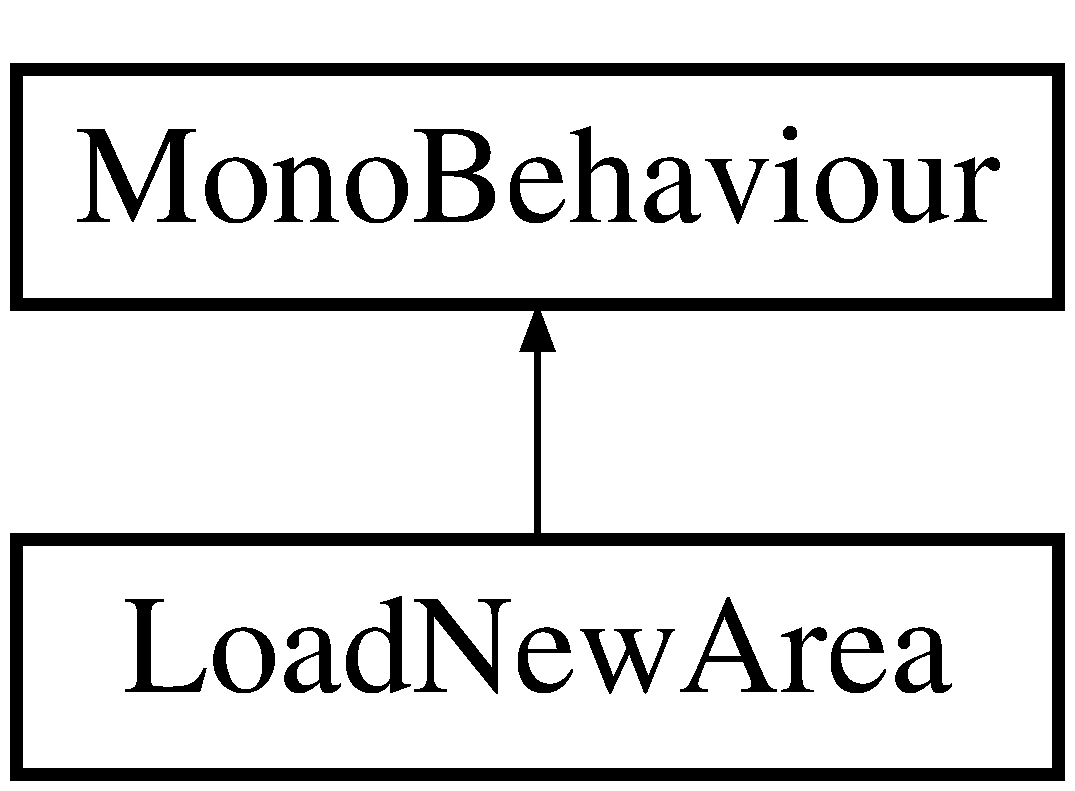
\includegraphics[height=2.000000cm]{class_load_new_area}
\end{center}
\end{figure}
\subsection*{Public Attributes}
\begin{DoxyCompactItemize}
\item 
\mbox{\Hypertarget{class_load_new_area_a1d4194f749b6ca5c9412d1185bb295e9}\label{class_load_new_area_a1d4194f749b6ca5c9412d1185bb295e9}} 
string {\bfseries level\+To\+Load}
\end{DoxyCompactItemize}
\subsection*{Private Member Functions}
\begin{DoxyCompactItemize}
\item 
\mbox{\Hypertarget{class_load_new_area_a2b5dd2fba10d61b23c375028b18eac22}\label{class_load_new_area_a2b5dd2fba10d61b23c375028b18eac22}} 
void {\bfseries Start} ()
\item 
\mbox{\Hypertarget{class_load_new_area_ae44863b1d524c2edab0732fefb815f06}\label{class_load_new_area_ae44863b1d524c2edab0732fefb815f06}} 
void {\bfseries Update} ()
\item 
void \mbox{\hyperlink{class_load_new_area_abdcf65c2a5ab9925bbd336e774baa82e}{On\+Trigger\+Enter2D}} (Collider2D other)
\begin{DoxyCompactList}\small\item\em This is the trigger for the door in between Levels 1 and 2 It requires the object passing through to be the player and the player must have collected all 4 items to move onto the next scene by making the trigger active \end{DoxyCompactList}\end{DoxyCompactItemize}


\subsection{Member Function Documentation}
\mbox{\Hypertarget{class_load_new_area_abdcf65c2a5ab9925bbd336e774baa82e}\label{class_load_new_area_abdcf65c2a5ab9925bbd336e774baa82e}} 
\index{Load\+New\+Area@{Load\+New\+Area}!On\+Trigger\+Enter2D@{On\+Trigger\+Enter2D}}
\index{On\+Trigger\+Enter2D@{On\+Trigger\+Enter2D}!Load\+New\+Area@{Load\+New\+Area}}
\subsubsection{\texorpdfstring{On\+Trigger\+Enter2\+D()}{OnTriggerEnter2D()}}
{\footnotesize\ttfamily void Load\+New\+Area.\+On\+Trigger\+Enter2D (\begin{DoxyParamCaption}\item[{Collider2D}]{other }\end{DoxyParamCaption})\hspace{0.3cm}{\ttfamily [private]}}



This is the trigger for the door in between Levels 1 and 2 It requires the object passing through to be the player and the player must have collected all 4 items to move onto the next scene by making the trigger active 


\begin{DoxyParams}{Parameters}
{\em other} & Other.\\
\hline
\end{DoxyParams}


The documentation for this class was generated from the following file\+:\begin{DoxyCompactItemize}
\item 
C\+:/\+Users/\+Am/\+Documents/\+Blue\+Shells -\/ Copy/\+Blue\+Shells/\+Seniors\+Gone\+Wild/\+Assets/\+Scripts/Load\+New\+Area.\+cs\end{DoxyCompactItemize}

\hypertarget{class_load_to_main}{}\section{Load\+To\+Main Class Reference}
\label{class_load_to_main}\index{Load\+To\+Main@{Load\+To\+Main}}
Inheritance diagram for Load\+To\+Main\+:\begin{figure}[H]
\begin{center}
\leavevmode
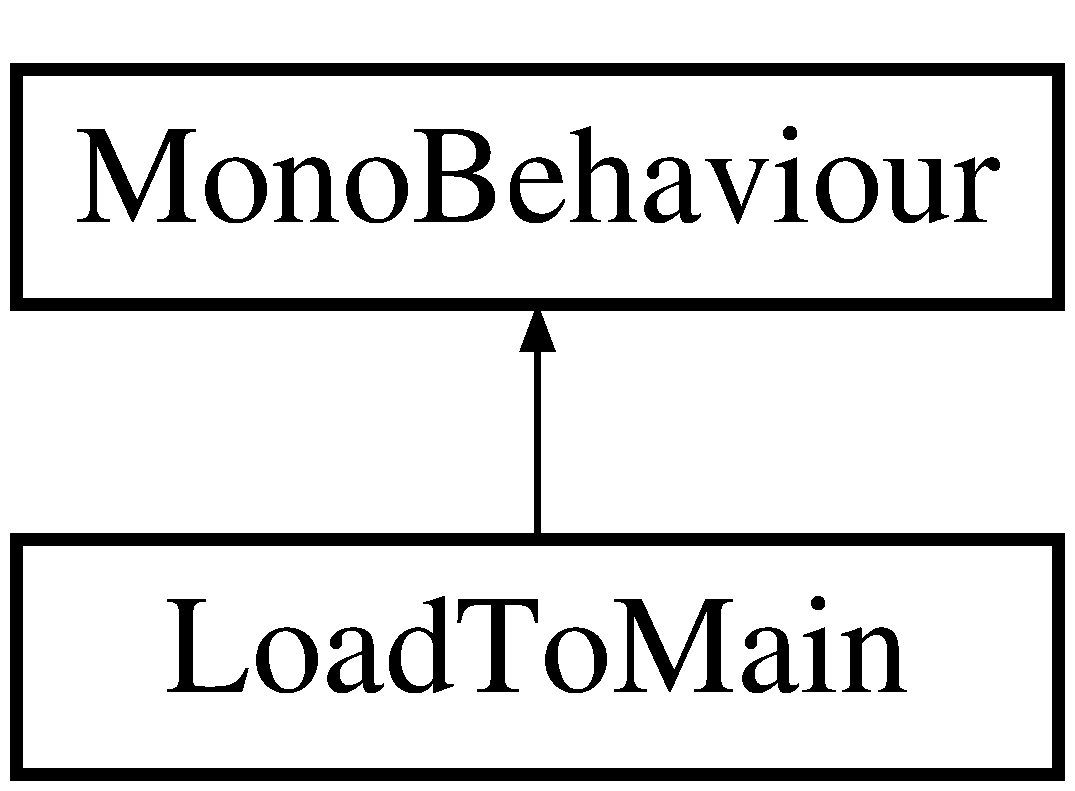
\includegraphics[height=2.000000cm]{class_load_to_main}
\end{center}
\end{figure}
\subsection*{Public Member Functions}
\begin{DoxyCompactItemize}
\item 
void \mbox{\hyperlink{class_load_to_main_a07eacdc3214c521d41e4ee14f9234a50}{Load\+Menu}} ()
\begin{DoxyCompactList}\small\item\em This function loads the menu from the End Scene \end{DoxyCompactList}\end{DoxyCompactItemize}


\subsection{Member Function Documentation}
\mbox{\Hypertarget{class_load_to_main_a07eacdc3214c521d41e4ee14f9234a50}\label{class_load_to_main_a07eacdc3214c521d41e4ee14f9234a50}} 
\index{Load\+To\+Main@{Load\+To\+Main}!Load\+Menu@{Load\+Menu}}
\index{Load\+Menu@{Load\+Menu}!Load\+To\+Main@{Load\+To\+Main}}
\subsubsection{\texorpdfstring{Load\+Menu()}{LoadMenu()}}
{\footnotesize\ttfamily void Load\+To\+Main.\+Load\+Menu (\begin{DoxyParamCaption}{ }\end{DoxyParamCaption})}



This function loads the menu from the End Scene 



The documentation for this class was generated from the following file\+:\begin{DoxyCompactItemize}
\item 
C\+:/\+Users/\+Am/\+Documents/\+Blue\+Shells -\/ Copy/\+Blue\+Shells/\+Seniors\+Gone\+Wild/\+Assets/\+Scripts/Load\+To\+Main.\+cs\end{DoxyCompactItemize}

\hypertarget{class_menu_script}{}\section{Menu\+Script Class Reference}
\label{class_menu_script}\index{Menu\+Script@{Menu\+Script}}
Inheritance diagram for Menu\+Script\+:\begin{figure}[H]
\begin{center}
\leavevmode
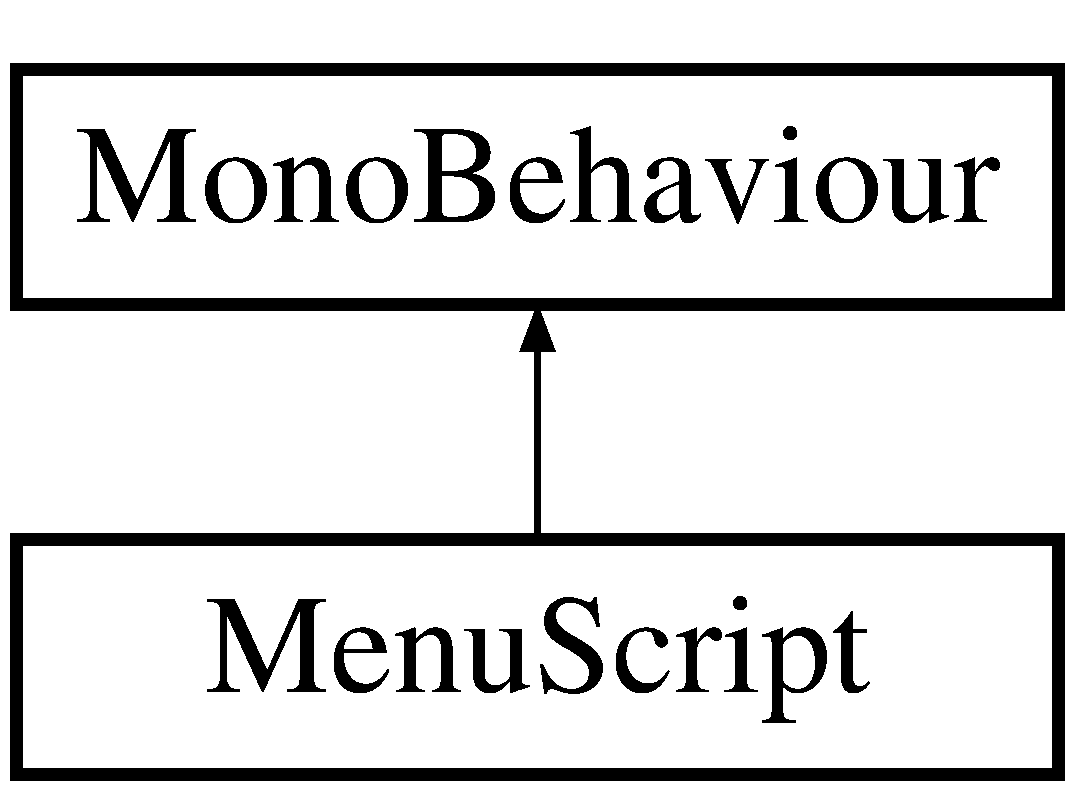
\includegraphics[height=2.000000cm]{class_menu_script}
\end{center}
\end{figure}
\subsection*{Public Member Functions}
\begin{DoxyCompactItemize}
\item 
void \mbox{\hyperlink{class_menu_script_a9347d5e7759ebceb5b1266faca8d336b}{Start\+Game}} ()
\begin{DoxyCompactList}\small\item\em Script attached to teh play button in Main\+Menu for starting the game at Level 1 \end{DoxyCompactList}\end{DoxyCompactItemize}


\subsection{Member Function Documentation}
\mbox{\Hypertarget{class_menu_script_a9347d5e7759ebceb5b1266faca8d336b}\label{class_menu_script_a9347d5e7759ebceb5b1266faca8d336b}} 
\index{Menu\+Script@{Menu\+Script}!Start\+Game@{Start\+Game}}
\index{Start\+Game@{Start\+Game}!Menu\+Script@{Menu\+Script}}
\subsubsection{\texorpdfstring{Start\+Game()}{StartGame()}}
{\footnotesize\ttfamily void Menu\+Script.\+Start\+Game (\begin{DoxyParamCaption}{ }\end{DoxyParamCaption})}



Script attached to teh play button in Main\+Menu for starting the game at Level 1 



The documentation for this class was generated from the following file\+:\begin{DoxyCompactItemize}
\item 
C\+:/\+Users/\+Am/\+Documents/\+Blue\+Shells -\/ Copy/\+Blue\+Shells/\+Seniors\+Gone\+Wild/\+Assets/\+Scripts/Menu\+Script.\+cs\end{DoxyCompactItemize}

\hypertarget{class_nurse_controller}{}\section{Nurse\+Controller Class Reference}
\label{class_nurse_controller}\index{Nurse\+Controller@{Nurse\+Controller}}
Inheritance diagram for Nurse\+Controller\+:\begin{figure}[H]
\begin{center}
\leavevmode
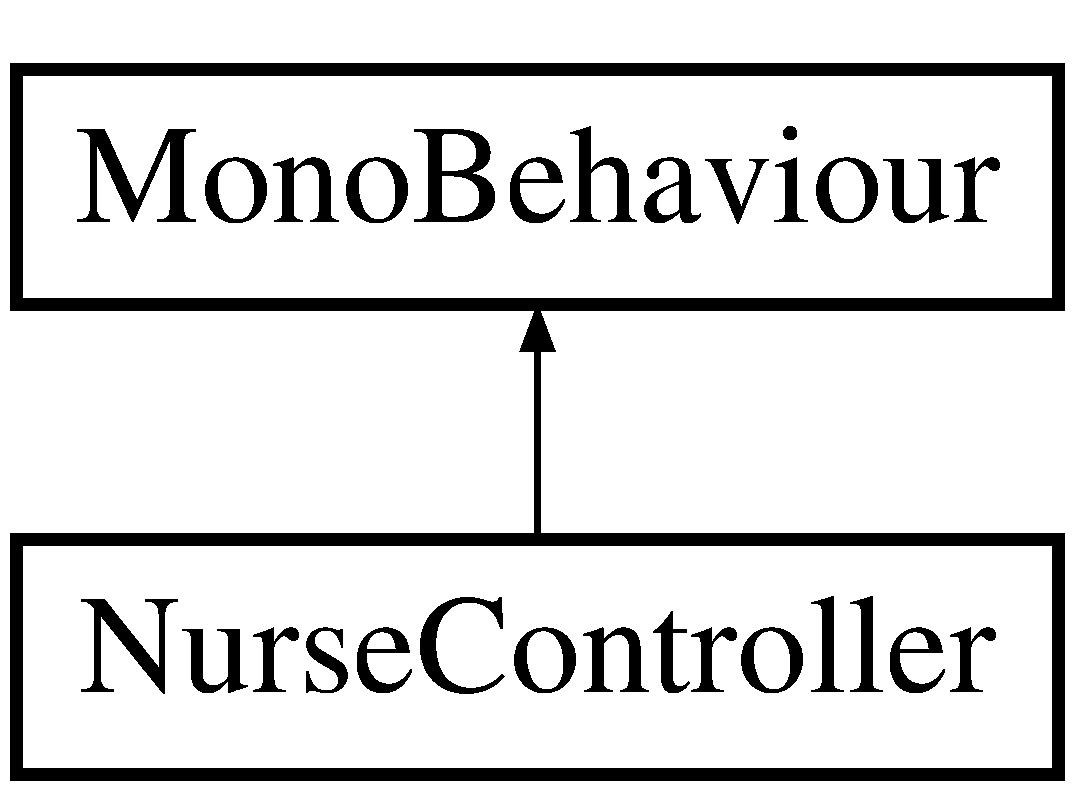
\includegraphics[height=2.000000cm]{class_nurse_controller}
\end{center}
\end{figure}
\subsection*{Public Attributes}
\begin{DoxyCompactItemize}
\item 
float \mbox{\hyperlink{class_nurse_controller_ac322ce98930aa447581ed2f996afa236}{move\+Speed}}
\begin{DoxyCompactList}\small\item\em Declares a moving speed for the nurse \end{DoxyCompactList}\item 
float \mbox{\hyperlink{class_nurse_controller_a2c526e24198abadb85a44b92c46a2fed}{time\+Between\+Move}}
\begin{DoxyCompactList}\small\item\em Because the nurse movement is random, the code needs a counter in between the randomized moves before the nurse will be set to move again \end{DoxyCompactList}\item 
float \mbox{\hyperlink{class_nurse_controller_a8d3c0f3a1e8e1b2082e98926c1e6ede6}{time\+To\+Move}}
\begin{DoxyCompactList}\small\item\em These set how long the nurse will be moving \end{DoxyCompactList}\item 
float \mbox{\hyperlink{class_nurse_controller_a75b6d8fbe22de1d605aff154528d9827}{wait\+To\+Beload}}
\begin{DoxyCompactList}\small\item\em This is for the character interation when caught by a nurse The character will reload, and there is a timer for that \end{DoxyCompactList}\end{DoxyCompactItemize}
\subsection*{Static Public Attributes}
\begin{DoxyCompactItemize}
\item 
static int \mbox{\hyperlink{class_nurse_controller_a02f9b6bcfd4d5082def13b1e69921b76}{score\+Count}} = 500
\begin{DoxyCompactList}\small\item\em This is used to set a baseline for the scoring system \end{DoxyCompactList}\end{DoxyCompactItemize}
\subsection*{Private Member Functions}
\begin{DoxyCompactItemize}
\item 
void \mbox{\hyperlink{class_nurse_controller_aa8fcc891957bbead5cfaa915045e3ded}{Start}} ()
\begin{DoxyCompactList}\small\item\em This function gives a rigid body to nurse It also sets a random time in between nurse movements \end{DoxyCompactList}\item 
void \mbox{\hyperlink{class_nurse_controller_a3c52dfb2cfa34450a3b0c379cbff1202}{Update}} ()
\begin{DoxyCompactList}\small\item\em If the time\+To\+Move\+Counter goes below zero, the nurse will stop moving for a random amount of time If the player is caught (wait\+To\+Beload $<$0), player will be reset to the beginning of the level and become active again \end{DoxyCompactList}\item 
void \mbox{\hyperlink{class_nurse_controller_a80a67354fb792c665c686f8b3ef4ba8d}{On\+Collision\+Enter2D}} (Collision2D other)
\begin{DoxyCompactList}\small\item\em If the player is caught by a nurse, he will become inactive and relaod. He will also have points added for every nurse contact. It also includes the sound that will be played on nurse contact. \end{DoxyCompactList}\end{DoxyCompactItemize}
\subsection*{Private Attributes}
\begin{DoxyCompactItemize}
\item 
Rigidbody2D \mbox{\hyperlink{class_nurse_controller_aa101cdff336129084914ac7b99c48dde}{my\+Rigid\+Body}}
\begin{DoxyCompactList}\small\item\em Declares a rigid body for the nurse \end{DoxyCompactList}\item 
bool \mbox{\hyperlink{class_nurse_controller_a51594c8ff5d4c71eeec6aef9fff4819c}{moving}}
\begin{DoxyCompactList}\small\item\em The nurse is either moving or is not \end{DoxyCompactList}\item 
\mbox{\Hypertarget{class_nurse_controller_a9bfdcd467ebbc3af37fe73001a4849c9}\label{class_nurse_controller_a9bfdcd467ebbc3af37fe73001a4849c9}} 
float {\bfseries time\+Between\+Move\+Counter}
\item 
\mbox{\Hypertarget{class_nurse_controller_a2c76f2ef1ad2679c9696608306ad533f}\label{class_nurse_controller_a2c76f2ef1ad2679c9696608306ad533f}} 
float {\bfseries time\+To\+Move\+Counter}
\item 
Vector3 \mbox{\hyperlink{class_nurse_controller_af1bbb9415d5e5fc25461cff6f72722f3}{move\+Direction}}
\begin{DoxyCompactList}\small\item\em Sets a moving direction for the nurse \end{DoxyCompactList}\item 
\mbox{\Hypertarget{class_nurse_controller_a7542b5de536e73a0aee7cb8a499ea055}\label{class_nurse_controller_a7542b5de536e73a0aee7cb8a499ea055}} 
bool {\bfseries reloading}
\item 
Game\+Object \mbox{\hyperlink{class_nurse_controller_a7977ec16f13d4a3b5b898ee479140a58}{the\+Player}}
\begin{DoxyCompactList}\small\item\em Includes the Player object \end{DoxyCompactList}\end{DoxyCompactItemize}


\subsection{Member Function Documentation}
\mbox{\Hypertarget{class_nurse_controller_a80a67354fb792c665c686f8b3ef4ba8d}\label{class_nurse_controller_a80a67354fb792c665c686f8b3ef4ba8d}} 
\index{Nurse\+Controller@{Nurse\+Controller}!On\+Collision\+Enter2D@{On\+Collision\+Enter2D}}
\index{On\+Collision\+Enter2D@{On\+Collision\+Enter2D}!Nurse\+Controller@{Nurse\+Controller}}
\subsubsection{\texorpdfstring{On\+Collision\+Enter2\+D()}{OnCollisionEnter2D()}}
{\footnotesize\ttfamily void Nurse\+Controller.\+On\+Collision\+Enter2D (\begin{DoxyParamCaption}\item[{Collision2D}]{other }\end{DoxyParamCaption})\hspace{0.3cm}{\ttfamily [private]}}



If the player is caught by a nurse, he will become inactive and relaod. He will also have points added for every nurse contact. It also includes the sound that will be played on nurse contact. 


\begin{DoxyParams}{Parameters}
{\em other} & Other.\\
\hline
\end{DoxyParams}
\mbox{\Hypertarget{class_nurse_controller_aa8fcc891957bbead5cfaa915045e3ded}\label{class_nurse_controller_aa8fcc891957bbead5cfaa915045e3ded}} 
\index{Nurse\+Controller@{Nurse\+Controller}!Start@{Start}}
\index{Start@{Start}!Nurse\+Controller@{Nurse\+Controller}}
\subsubsection{\texorpdfstring{Start()}{Start()}}
{\footnotesize\ttfamily void Nurse\+Controller.\+Start (\begin{DoxyParamCaption}{ }\end{DoxyParamCaption})\hspace{0.3cm}{\ttfamily [private]}}



This function gives a rigid body to nurse It also sets a random time in between nurse movements 

\mbox{\Hypertarget{class_nurse_controller_a3c52dfb2cfa34450a3b0c379cbff1202}\label{class_nurse_controller_a3c52dfb2cfa34450a3b0c379cbff1202}} 
\index{Nurse\+Controller@{Nurse\+Controller}!Update@{Update}}
\index{Update@{Update}!Nurse\+Controller@{Nurse\+Controller}}
\subsubsection{\texorpdfstring{Update()}{Update()}}
{\footnotesize\ttfamily void Nurse\+Controller.\+Update (\begin{DoxyParamCaption}{ }\end{DoxyParamCaption})\hspace{0.3cm}{\ttfamily [private]}}



If the time\+To\+Move\+Counter goes below zero, the nurse will stop moving for a random amount of time If the player is caught (wait\+To\+Beload $<$0), player will be reset to the beginning of the level and become active again 



\subsection{Member Data Documentation}
\mbox{\Hypertarget{class_nurse_controller_af1bbb9415d5e5fc25461cff6f72722f3}\label{class_nurse_controller_af1bbb9415d5e5fc25461cff6f72722f3}} 
\index{Nurse\+Controller@{Nurse\+Controller}!move\+Direction@{move\+Direction}}
\index{move\+Direction@{move\+Direction}!Nurse\+Controller@{Nurse\+Controller}}
\subsubsection{\texorpdfstring{move\+Direction}{moveDirection}}
{\footnotesize\ttfamily Vector3 Nurse\+Controller.\+move\+Direction\hspace{0.3cm}{\ttfamily [private]}}



Sets a moving direction for the nurse 

\mbox{\Hypertarget{class_nurse_controller_ac322ce98930aa447581ed2f996afa236}\label{class_nurse_controller_ac322ce98930aa447581ed2f996afa236}} 
\index{Nurse\+Controller@{Nurse\+Controller}!move\+Speed@{move\+Speed}}
\index{move\+Speed@{move\+Speed}!Nurse\+Controller@{Nurse\+Controller}}
\subsubsection{\texorpdfstring{move\+Speed}{moveSpeed}}
{\footnotesize\ttfamily float Nurse\+Controller.\+move\+Speed}



Declares a moving speed for the nurse 

\mbox{\Hypertarget{class_nurse_controller_a51594c8ff5d4c71eeec6aef9fff4819c}\label{class_nurse_controller_a51594c8ff5d4c71eeec6aef9fff4819c}} 
\index{Nurse\+Controller@{Nurse\+Controller}!moving@{moving}}
\index{moving@{moving}!Nurse\+Controller@{Nurse\+Controller}}
\subsubsection{\texorpdfstring{moving}{moving}}
{\footnotesize\ttfamily bool Nurse\+Controller.\+moving\hspace{0.3cm}{\ttfamily [private]}}



The nurse is either moving or is not 

\mbox{\Hypertarget{class_nurse_controller_aa101cdff336129084914ac7b99c48dde}\label{class_nurse_controller_aa101cdff336129084914ac7b99c48dde}} 
\index{Nurse\+Controller@{Nurse\+Controller}!my\+Rigid\+Body@{my\+Rigid\+Body}}
\index{my\+Rigid\+Body@{my\+Rigid\+Body}!Nurse\+Controller@{Nurse\+Controller}}
\subsubsection{\texorpdfstring{my\+Rigid\+Body}{myRigidBody}}
{\footnotesize\ttfamily Rigidbody2D Nurse\+Controller.\+my\+Rigid\+Body\hspace{0.3cm}{\ttfamily [private]}}



Declares a rigid body for the nurse 

\mbox{\Hypertarget{class_nurse_controller_a02f9b6bcfd4d5082def13b1e69921b76}\label{class_nurse_controller_a02f9b6bcfd4d5082def13b1e69921b76}} 
\index{Nurse\+Controller@{Nurse\+Controller}!score\+Count@{score\+Count}}
\index{score\+Count@{score\+Count}!Nurse\+Controller@{Nurse\+Controller}}
\subsubsection{\texorpdfstring{score\+Count}{scoreCount}}
{\footnotesize\ttfamily int Nurse\+Controller.\+score\+Count = 500\hspace{0.3cm}{\ttfamily [static]}}



This is used to set a baseline for the scoring system 

\mbox{\Hypertarget{class_nurse_controller_a7977ec16f13d4a3b5b898ee479140a58}\label{class_nurse_controller_a7977ec16f13d4a3b5b898ee479140a58}} 
\index{Nurse\+Controller@{Nurse\+Controller}!the\+Player@{the\+Player}}
\index{the\+Player@{the\+Player}!Nurse\+Controller@{Nurse\+Controller}}
\subsubsection{\texorpdfstring{the\+Player}{thePlayer}}
{\footnotesize\ttfamily Game\+Object Nurse\+Controller.\+the\+Player\hspace{0.3cm}{\ttfamily [private]}}



Includes the Player object 

\mbox{\Hypertarget{class_nurse_controller_a2c526e24198abadb85a44b92c46a2fed}\label{class_nurse_controller_a2c526e24198abadb85a44b92c46a2fed}} 
\index{Nurse\+Controller@{Nurse\+Controller}!time\+Between\+Move@{time\+Between\+Move}}
\index{time\+Between\+Move@{time\+Between\+Move}!Nurse\+Controller@{Nurse\+Controller}}
\subsubsection{\texorpdfstring{time\+Between\+Move}{timeBetweenMove}}
{\footnotesize\ttfamily float Nurse\+Controller.\+time\+Between\+Move}



Because the nurse movement is random, the code needs a counter in between the randomized moves before the nurse will be set to move again 

\mbox{\Hypertarget{class_nurse_controller_a8d3c0f3a1e8e1b2082e98926c1e6ede6}\label{class_nurse_controller_a8d3c0f3a1e8e1b2082e98926c1e6ede6}} 
\index{Nurse\+Controller@{Nurse\+Controller}!time\+To\+Move@{time\+To\+Move}}
\index{time\+To\+Move@{time\+To\+Move}!Nurse\+Controller@{Nurse\+Controller}}
\subsubsection{\texorpdfstring{time\+To\+Move}{timeToMove}}
{\footnotesize\ttfamily float Nurse\+Controller.\+time\+To\+Move}



These set how long the nurse will be moving 

\mbox{\Hypertarget{class_nurse_controller_a75b6d8fbe22de1d605aff154528d9827}\label{class_nurse_controller_a75b6d8fbe22de1d605aff154528d9827}} 
\index{Nurse\+Controller@{Nurse\+Controller}!wait\+To\+Beload@{wait\+To\+Beload}}
\index{wait\+To\+Beload@{wait\+To\+Beload}!Nurse\+Controller@{Nurse\+Controller}}
\subsubsection{\texorpdfstring{wait\+To\+Beload}{waitToBeload}}
{\footnotesize\ttfamily float Nurse\+Controller.\+wait\+To\+Beload}



This is for the character interation when caught by a nurse The character will reload, and there is a timer for that 



The documentation for this class was generated from the following file\+:\begin{DoxyCompactItemize}
\item 
C\+:/\+Users/\+Am/\+Documents/\+Blue\+Shells -\/ Copy/\+Blue\+Shells/\+Seniors\+Gone\+Wild/\+Assets/\+Scripts/Nurse\+Controller.\+cs\end{DoxyCompactItemize}

\hypertarget{class_player_controller}{}\section{Player\+Controller Class Reference}
\label{class_player_controller}\index{Player\+Controller@{Player\+Controller}}
Inheritance diagram for Player\+Controller\+:\begin{figure}[H]
\begin{center}
\leavevmode
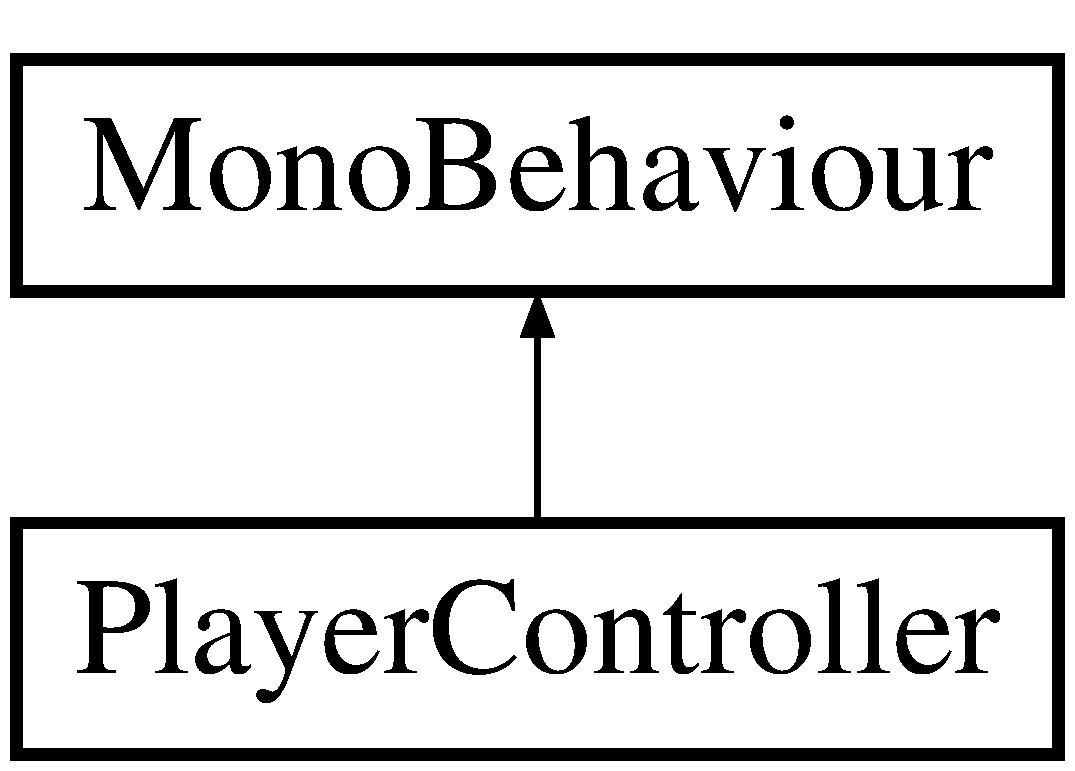
\includegraphics[height=2.000000cm]{class_player_controller}
\end{center}
\end{figure}
\subsection*{Public Attributes}
\begin{DoxyCompactItemize}
\item 
float \mbox{\hyperlink{class_player_controller_abb12e85ca1b12efdbc8684bff2e19c4c}{move\+Speed}}
\begin{DoxyCompactList}\small\item\em Creates move speed for player \end{DoxyCompactList}\item 
\mbox{\Hypertarget{class_player_controller_a8734946783cad257b722f45fe4af8c6c}\label{class_player_controller_a8734946783cad257b722f45fe4af8c6c}} 
Vector2 {\bfseries last\+Move}
\item 
\mbox{\Hypertarget{class_player_controller_a61795bee5f0ca4705f688419919e3086}\label{class_player_controller_a61795bee5f0ca4705f688419919e3086}} 
Text {\bfseries count\+Text}
\item 
\mbox{\Hypertarget{class_player_controller_a366f431ae274e7b19365f7b15b1709b8}\label{class_player_controller_a366f431ae274e7b19365f7b15b1709b8}} 
Text {\bfseries win\+Text}
\item 
bool \mbox{\hyperlink{class_player_controller_a14bb057d727180f87728bd6fe62dffc9}{can\+Move}}
\begin{DoxyCompactList}\small\item\em Variable for pausing movement during dialogue \end{DoxyCompactList}\end{DoxyCompactItemize}
\subsection*{Static Public Attributes}
\begin{DoxyCompactItemize}
\item 
static int \mbox{\hyperlink{class_player_controller_a0e233eee5112d304b1bb5a118d6087e7}{item\+Count}}
\begin{DoxyCompactList}\small\item\em These variables are used to keep track of item collection \end{DoxyCompactList}\end{DoxyCompactItemize}
\subsection*{Private Member Functions}
\begin{DoxyCompactItemize}
\item 
void \mbox{\hyperlink{class_player_controller_ae1117d9c4da3193181cddad2c814e467}{Start}} ()
\begin{DoxyCompactList}\small\item\em Item count is set to zero when the game starts and will display no win text until later If the player doesn\textquotesingle{}t exist, it creates a player Otherwise, if there is a player, the player is destroyed and replaced This is used for movement to the next scene \end{DoxyCompactList}\item 
void \mbox{\hyperlink{class_player_controller_ae8bc83dffb99867a04be016473ed2c43}{Update}} ()
\begin{DoxyCompactList}\small\item\em This function is used to pause the character\textquotesingle{}s movement while dialogue is open By default, the player is static until given input Based on the keys pressed, the player will either move horizontally or vertically and will retain the direction of it\textquotesingle{}s last move until a directional button is pushed again \end{DoxyCompactList}\item 
void \mbox{\hyperlink{class_player_controller_a751c7590dfb8e726d1eb3a27d0b197a2}{On\+Trigger\+Enter2D}} (Collider2D other)
\begin{DoxyCompactList}\small\item\em If items are collected, 1 is added to the count A sound will be played upon item collection \end{DoxyCompactList}\item 
void \mbox{\hyperlink{class_player_controller_ad55b05bf5e6a5ae39a2a01700f1772ce}{Set\+Count\+Text}} ()
\begin{DoxyCompactList}\small\item\em This function displays a text that shows the amount of iems collected If the item amount is equal to 4 or greater, display \char`\"{}win and escape\char`\"{} text \end{DoxyCompactList}\end{DoxyCompactItemize}
\subsection*{Private Attributes}
\begin{DoxyCompactItemize}
\item 
Animator \mbox{\hyperlink{class_player_controller_ac646d94772588e3393eb5cb9ac02a5c4}{anim}}
\begin{DoxyCompactList}\small\item\em Inlcudes the animations for the player and creates a rigidbody \end{DoxyCompactList}\item 
\mbox{\Hypertarget{class_player_controller_a87b5271776e29f73db019d63a639c234}\label{class_player_controller_a87b5271776e29f73db019d63a639c234}} 
Rigidbody2D {\bfseries my\+Rigidbody}
\item 
bool \mbox{\hyperlink{class_player_controller_a15143b0b40abe525495279ea3cd4ba82}{player\+Moving}}
\begin{DoxyCompactList}\small\item\em Player is either moving or is not \end{DoxyCompactList}\end{DoxyCompactItemize}
\subsection*{Static Private Attributes}
\begin{DoxyCompactItemize}
\item 
static bool \mbox{\hyperlink{class_player_controller_aee578ffd54e0e8e2f8149e2d3d1ba036}{player\+Exists}}
\begin{DoxyCompactList}\small\item\em Player either exists or does not \end{DoxyCompactList}\end{DoxyCompactItemize}


\subsection{Member Function Documentation}
\mbox{\Hypertarget{class_player_controller_a751c7590dfb8e726d1eb3a27d0b197a2}\label{class_player_controller_a751c7590dfb8e726d1eb3a27d0b197a2}} 
\index{Player\+Controller@{Player\+Controller}!On\+Trigger\+Enter2D@{On\+Trigger\+Enter2D}}
\index{On\+Trigger\+Enter2D@{On\+Trigger\+Enter2D}!Player\+Controller@{Player\+Controller}}
\subsubsection{\texorpdfstring{On\+Trigger\+Enter2\+D()}{OnTriggerEnter2D()}}
{\footnotesize\ttfamily void Player\+Controller.\+On\+Trigger\+Enter2D (\begin{DoxyParamCaption}\item[{Collider2D}]{other }\end{DoxyParamCaption})\hspace{0.3cm}{\ttfamily [private]}}



If items are collected, 1 is added to the count A sound will be played upon item collection 


\begin{DoxyParams}{Parameters}
{\em other} & Other.\\
\hline
\end{DoxyParams}
\mbox{\Hypertarget{class_player_controller_ad55b05bf5e6a5ae39a2a01700f1772ce}\label{class_player_controller_ad55b05bf5e6a5ae39a2a01700f1772ce}} 
\index{Player\+Controller@{Player\+Controller}!Set\+Count\+Text@{Set\+Count\+Text}}
\index{Set\+Count\+Text@{Set\+Count\+Text}!Player\+Controller@{Player\+Controller}}
\subsubsection{\texorpdfstring{Set\+Count\+Text()}{SetCountText()}}
{\footnotesize\ttfamily void Player\+Controller.\+Set\+Count\+Text (\begin{DoxyParamCaption}{ }\end{DoxyParamCaption})\hspace{0.3cm}{\ttfamily [private]}}



This function displays a text that shows the amount of iems collected If the item amount is equal to 4 or greater, display \char`\"{}win and escape\char`\"{} text 

\mbox{\Hypertarget{class_player_controller_ae1117d9c4da3193181cddad2c814e467}\label{class_player_controller_ae1117d9c4da3193181cddad2c814e467}} 
\index{Player\+Controller@{Player\+Controller}!Start@{Start}}
\index{Start@{Start}!Player\+Controller@{Player\+Controller}}
\subsubsection{\texorpdfstring{Start()}{Start()}}
{\footnotesize\ttfamily void Player\+Controller.\+Start (\begin{DoxyParamCaption}{ }\end{DoxyParamCaption})\hspace{0.3cm}{\ttfamily [private]}}



Item count is set to zero when the game starts and will display no win text until later If the player doesn\textquotesingle{}t exist, it creates a player Otherwise, if there is a player, the player is destroyed and replaced This is used for movement to the next scene 

\mbox{\Hypertarget{class_player_controller_ae8bc83dffb99867a04be016473ed2c43}\label{class_player_controller_ae8bc83dffb99867a04be016473ed2c43}} 
\index{Player\+Controller@{Player\+Controller}!Update@{Update}}
\index{Update@{Update}!Player\+Controller@{Player\+Controller}}
\subsubsection{\texorpdfstring{Update()}{Update()}}
{\footnotesize\ttfamily void Player\+Controller.\+Update (\begin{DoxyParamCaption}{ }\end{DoxyParamCaption})\hspace{0.3cm}{\ttfamily [private]}}



This function is used to pause the character\textquotesingle{}s movement while dialogue is open By default, the player is static until given input Based on the keys pressed, the player will either move horizontally or vertically and will retain the direction of it\textquotesingle{}s last move until a directional button is pushed again 



\subsection{Member Data Documentation}
\mbox{\Hypertarget{class_player_controller_ac646d94772588e3393eb5cb9ac02a5c4}\label{class_player_controller_ac646d94772588e3393eb5cb9ac02a5c4}} 
\index{Player\+Controller@{Player\+Controller}!anim@{anim}}
\index{anim@{anim}!Player\+Controller@{Player\+Controller}}
\subsubsection{\texorpdfstring{anim}{anim}}
{\footnotesize\ttfamily Animator Player\+Controller.\+anim\hspace{0.3cm}{\ttfamily [private]}}



Inlcudes the animations for the player and creates a rigidbody 

\mbox{\Hypertarget{class_player_controller_a14bb057d727180f87728bd6fe62dffc9}\label{class_player_controller_a14bb057d727180f87728bd6fe62dffc9}} 
\index{Player\+Controller@{Player\+Controller}!can\+Move@{can\+Move}}
\index{can\+Move@{can\+Move}!Player\+Controller@{Player\+Controller}}
\subsubsection{\texorpdfstring{can\+Move}{canMove}}
{\footnotesize\ttfamily bool Player\+Controller.\+can\+Move}



Variable for pausing movement during dialogue 

\mbox{\Hypertarget{class_player_controller_a0e233eee5112d304b1bb5a118d6087e7}\label{class_player_controller_a0e233eee5112d304b1bb5a118d6087e7}} 
\index{Player\+Controller@{Player\+Controller}!item\+Count@{item\+Count}}
\index{item\+Count@{item\+Count}!Player\+Controller@{Player\+Controller}}
\subsubsection{\texorpdfstring{item\+Count}{itemCount}}
{\footnotesize\ttfamily int Player\+Controller.\+item\+Count\hspace{0.3cm}{\ttfamily [static]}}



These variables are used to keep track of item collection 

\mbox{\Hypertarget{class_player_controller_abb12e85ca1b12efdbc8684bff2e19c4c}\label{class_player_controller_abb12e85ca1b12efdbc8684bff2e19c4c}} 
\index{Player\+Controller@{Player\+Controller}!move\+Speed@{move\+Speed}}
\index{move\+Speed@{move\+Speed}!Player\+Controller@{Player\+Controller}}
\subsubsection{\texorpdfstring{move\+Speed}{moveSpeed}}
{\footnotesize\ttfamily float Player\+Controller.\+move\+Speed}



Creates move speed for player 

\mbox{\Hypertarget{class_player_controller_aee578ffd54e0e8e2f8149e2d3d1ba036}\label{class_player_controller_aee578ffd54e0e8e2f8149e2d3d1ba036}} 
\index{Player\+Controller@{Player\+Controller}!player\+Exists@{player\+Exists}}
\index{player\+Exists@{player\+Exists}!Player\+Controller@{Player\+Controller}}
\subsubsection{\texorpdfstring{player\+Exists}{playerExists}}
{\footnotesize\ttfamily bool Player\+Controller.\+player\+Exists\hspace{0.3cm}{\ttfamily [static]}, {\ttfamily [private]}}



Player either exists or does not 

\mbox{\Hypertarget{class_player_controller_a15143b0b40abe525495279ea3cd4ba82}\label{class_player_controller_a15143b0b40abe525495279ea3cd4ba82}} 
\index{Player\+Controller@{Player\+Controller}!player\+Moving@{player\+Moving}}
\index{player\+Moving@{player\+Moving}!Player\+Controller@{Player\+Controller}}
\subsubsection{\texorpdfstring{player\+Moving}{playerMoving}}
{\footnotesize\ttfamily bool Player\+Controller.\+player\+Moving\hspace{0.3cm}{\ttfamily [private]}}



Player is either moving or is not 



The documentation for this class was generated from the following file\+:\begin{DoxyCompactItemize}
\item 
C\+:/\+Users/\+Am/\+Documents/\+Blue\+Shells -\/ Copy/\+Blue\+Shells/\+Seniors\+Gone\+Wild/\+Assets/\+Scripts/Player\+Controller.\+cs\end{DoxyCompactItemize}

\hypertarget{class_player_start_point}{}\section{Player\+Start\+Point Class Reference}
\label{class_player_start_point}\index{Player\+Start\+Point@{Player\+Start\+Point}}
Inheritance diagram for Player\+Start\+Point\+:\begin{figure}[H]
\begin{center}
\leavevmode
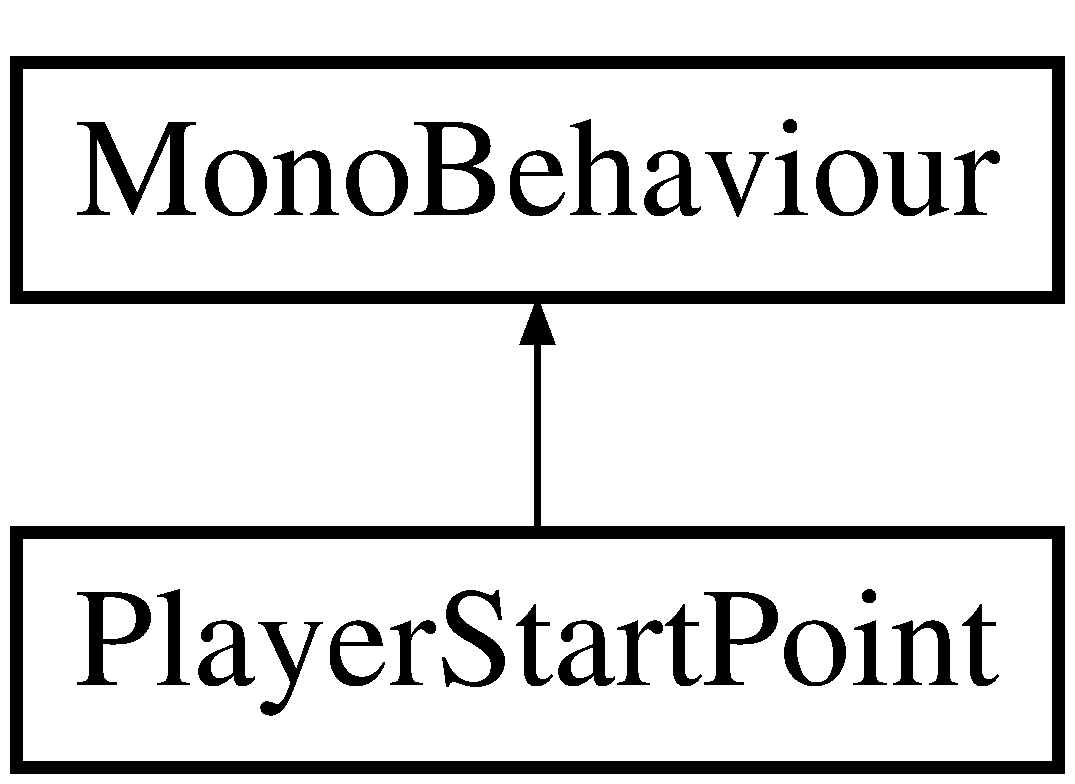
\includegraphics[height=2.000000cm]{class_player_start_point}
\end{center}
\end{figure}
\subsection*{Public Attributes}
\begin{DoxyCompactItemize}
\item 
Vector2 \mbox{\hyperlink{class_player_start_point_abdc8a9f45e6064dad9a93c60e29a4832}{start\+Direction}}
\begin{DoxyCompactList}\small\item\em Creates the starting direction \end{DoxyCompactList}\end{DoxyCompactItemize}
\subsection*{Private Member Functions}
\begin{DoxyCompactItemize}
\item 
void \mbox{\hyperlink{class_player_start_point_a54401d0571e76bb7a7a3161a0147b787}{Start}} ()
\begin{DoxyCompactList}\small\item\em This function finds the player, and uses the last move to set the new direction in the next level It also sets the camera in the same position post-\/level transition \end{DoxyCompactList}\item 
\mbox{\Hypertarget{class_player_start_point_adff99d06947271bc2275741911f659b1}\label{class_player_start_point_adff99d06947271bc2275741911f659b1}} 
void {\bfseries Update} ()
\end{DoxyCompactItemize}
\subsection*{Private Attributes}
\begin{DoxyCompactItemize}
\item 
\mbox{\hyperlink{class_player_controller}{Player\+Controller}} \mbox{\hyperlink{class_player_start_point_a4242b06d9f40b1729a83ffb3508772c4}{the\+Player}}
\begin{DoxyCompactList}\small\item\em Uses the player and camera controllers \end{DoxyCompactList}\item 
\mbox{\Hypertarget{class_player_start_point_af4e288ae79aa800dfeb6ca7013052db1}\label{class_player_start_point_af4e288ae79aa800dfeb6ca7013052db1}} 
\mbox{\hyperlink{class_camera_controller}{Camera\+Controller}} {\bfseries the\+Camera}
\end{DoxyCompactItemize}


\subsection{Member Function Documentation}
\mbox{\Hypertarget{class_player_start_point_a54401d0571e76bb7a7a3161a0147b787}\label{class_player_start_point_a54401d0571e76bb7a7a3161a0147b787}} 
\index{Player\+Start\+Point@{Player\+Start\+Point}!Start@{Start}}
\index{Start@{Start}!Player\+Start\+Point@{Player\+Start\+Point}}
\subsubsection{\texorpdfstring{Start()}{Start()}}
{\footnotesize\ttfamily void Player\+Start\+Point.\+Start (\begin{DoxyParamCaption}{ }\end{DoxyParamCaption})\hspace{0.3cm}{\ttfamily [private]}}



This function finds the player, and uses the last move to set the new direction in the next level It also sets the camera in the same position post-\/level transition 



\subsection{Member Data Documentation}
\mbox{\Hypertarget{class_player_start_point_abdc8a9f45e6064dad9a93c60e29a4832}\label{class_player_start_point_abdc8a9f45e6064dad9a93c60e29a4832}} 
\index{Player\+Start\+Point@{Player\+Start\+Point}!start\+Direction@{start\+Direction}}
\index{start\+Direction@{start\+Direction}!Player\+Start\+Point@{Player\+Start\+Point}}
\subsubsection{\texorpdfstring{start\+Direction}{startDirection}}
{\footnotesize\ttfamily Vector2 Player\+Start\+Point.\+start\+Direction}



Creates the starting direction 

\mbox{\Hypertarget{class_player_start_point_a4242b06d9f40b1729a83ffb3508772c4}\label{class_player_start_point_a4242b06d9f40b1729a83ffb3508772c4}} 
\index{Player\+Start\+Point@{Player\+Start\+Point}!the\+Player@{the\+Player}}
\index{the\+Player@{the\+Player}!Player\+Start\+Point@{Player\+Start\+Point}}
\subsubsection{\texorpdfstring{the\+Player}{thePlayer}}
{\footnotesize\ttfamily \mbox{\hyperlink{class_player_controller}{Player\+Controller}} Player\+Start\+Point.\+the\+Player\hspace{0.3cm}{\ttfamily [private]}}



Uses the player and camera controllers 



The documentation for this class was generated from the following file\+:\begin{DoxyCompactItemize}
\item 
C\+:/\+Users/\+Am/\+Documents/\+Blue\+Shells -\/ Copy/\+Blue\+Shells/\+Seniors\+Gone\+Wild/\+Assets/\+Scripts/Player\+Start\+Point.\+cs\end{DoxyCompactItemize}

\hypertarget{class_quit_button}{}\section{Quit\+Button Class Reference}
\label{class_quit_button}\index{Quit\+Button@{Quit\+Button}}
Inheritance diagram for Quit\+Button\+:\begin{figure}[H]
\begin{center}
\leavevmode
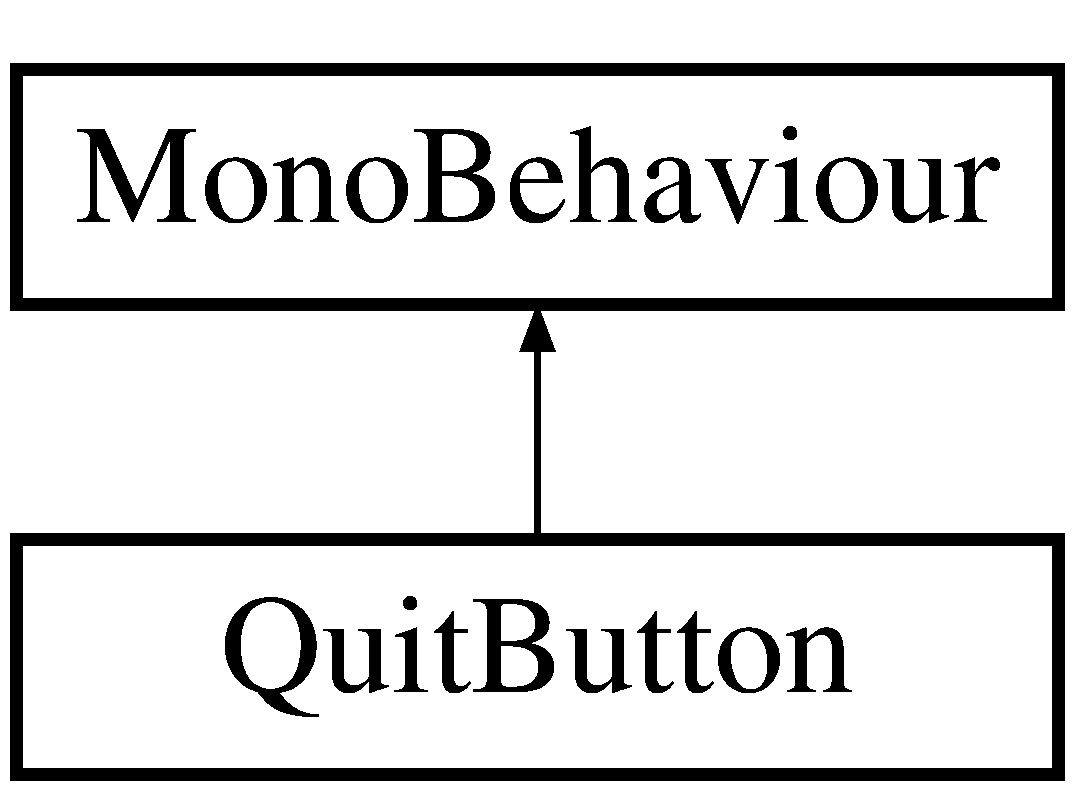
\includegraphics[height=2.000000cm]{class_quit_button}
\end{center}
\end{figure}
\subsection*{Public Member Functions}
\begin{DoxyCompactItemize}
\item 
void \mbox{\hyperlink{class_quit_button_ad8a6d288733d21c2376a31fb8df7b0ac}{Exit\+Game}} ()
\begin{DoxyCompactList}\small\item\em This function attaches to the quit button in the Main\+Menu used for exiting the game entirely \end{DoxyCompactList}\end{DoxyCompactItemize}


\subsection{Member Function Documentation}
\mbox{\Hypertarget{class_quit_button_ad8a6d288733d21c2376a31fb8df7b0ac}\label{class_quit_button_ad8a6d288733d21c2376a31fb8df7b0ac}} 
\index{Quit\+Button@{Quit\+Button}!Exit\+Game@{Exit\+Game}}
\index{Exit\+Game@{Exit\+Game}!Quit\+Button@{Quit\+Button}}
\subsubsection{\texorpdfstring{Exit\+Game()}{ExitGame()}}
{\footnotesize\ttfamily void Quit\+Button.\+Exit\+Game (\begin{DoxyParamCaption}{ }\end{DoxyParamCaption})}



This function attaches to the quit button in the Main\+Menu used for exiting the game entirely 



The documentation for this class was generated from the following file\+:\begin{DoxyCompactItemize}
\item 
C\+:/\+Users/\+Am/\+Documents/\+Blue\+Shells -\/ Copy/\+Blue\+Shells/\+Seniors\+Gone\+Wild/\+Assets/\+Scripts/Quit\+Button.\+cs\end{DoxyCompactItemize}

\hypertarget{class_sound}{}\section{Sound Class Reference}
\label{class_sound}\index{Sound@{Sound}}


This is necessary for getting access to audio settings like volume and pitch this will give this class a permission to appear in the inspector  


\subsection*{Public Attributes}
\begin{DoxyCompactItemize}
\item 
string \mbox{\hyperlink{class_sound_a6232daa7d1f983315cc0d10cf776ab76}{name}}
\begin{DoxyCompactList}\small\item\em Creates a name and a clip variables to be used in Unity \end{DoxyCompactList}\item 
\mbox{\Hypertarget{class_sound_ab7878c271c13d5e8fbdf25714e363b77}\label{class_sound_ab7878c271c13d5e8fbdf25714e363b77}} 
Audio\+Clip {\bfseries clip}
\item 
float \mbox{\hyperlink{class_sound_a7ab1335f27bd340c389568889823cc00}{volume}}
\begin{DoxyCompactList}\small\item\em these are minimum and maximum values \end{DoxyCompactList}\item 
\mbox{\Hypertarget{class_sound_aef4ee55185bf12b9b2b2ca037a8c621a}\label{class_sound_aef4ee55185bf12b9b2b2ca037a8c621a}} 
float {\bfseries pitch}
\item 
bool \mbox{\hyperlink{class_sound_a24f0da6a226712e28b3159aa9ebb4be5}{loop}}
\begin{DoxyCompactList}\small\item\em this will hide the variable from the Inspector. We do this because this is a value that we publish automatically in the awake method \end{DoxyCompactList}\item 
\mbox{\Hypertarget{class_sound_ac6ec734812a52abf31595cab2ba48d8d}\label{class_sound_ac6ec734812a52abf31595cab2ba48d8d}} 
Audio\+Source {\bfseries source}
\end{DoxyCompactItemize}


\subsection{Detailed Description}
This is necessary for getting access to audio settings like volume and pitch this will give this class a permission to appear in the inspector 



\subsection{Member Data Documentation}
\mbox{\Hypertarget{class_sound_a24f0da6a226712e28b3159aa9ebb4be5}\label{class_sound_a24f0da6a226712e28b3159aa9ebb4be5}} 
\index{Sound@{Sound}!loop@{loop}}
\index{loop@{loop}!Sound@{Sound}}
\subsubsection{\texorpdfstring{loop}{loop}}
{\footnotesize\ttfamily bool Sound.\+loop}



this will hide the variable from the Inspector. We do this because this is a value that we publish automatically in the awake method 

\mbox{\Hypertarget{class_sound_a6232daa7d1f983315cc0d10cf776ab76}\label{class_sound_a6232daa7d1f983315cc0d10cf776ab76}} 
\index{Sound@{Sound}!name@{name}}
\index{name@{name}!Sound@{Sound}}
\subsubsection{\texorpdfstring{name}{name}}
{\footnotesize\ttfamily string Sound.\+name}



Creates a name and a clip variables to be used in Unity 

\mbox{\Hypertarget{class_sound_a7ab1335f27bd340c389568889823cc00}\label{class_sound_a7ab1335f27bd340c389568889823cc00}} 
\index{Sound@{Sound}!volume@{volume}}
\index{volume@{volume}!Sound@{Sound}}
\subsubsection{\texorpdfstring{volume}{volume}}
{\footnotesize\ttfamily float Sound.\+volume}



these are minimum and maximum values 



The documentation for this class was generated from the following file\+:\begin{DoxyCompactItemize}
\item 
C\+:/\+Users/\+Am/\+Documents/\+Blue\+Shells -\/ Copy/\+Blue\+Shells/\+Seniors\+Gone\+Wild/\+Assets/\+Scripts/Sound.\+cs\end{DoxyCompactItemize}

%--- End generated contents ---

% Index
\backmatter
\newpage
\phantomsection
\clearemptydoublepage
\addcontentsline{toc}{chapter}{Index}
\printindex

\end{document}
